\subsection{Separation}
\label{sec:mathpro:steady:sep}
    \todo{find appropriate place for integrated reboiler condenser unit.}
    \todo{add flowsheet initialization from MathModel file}
        The separation step within the process occurs within a double effect distillation column.
    Distillation columns are among the most widely studied pieces of process equipment. While much has been
    accomplished, the robust simulation poses great challenges to this day. In the context of cryogenic
    air separation the associated mixture displays only moderate non-idealities and furthermore is
    a zeotropic one. However further complexity is added due to the strong interdependencies of the different
    columns arising from thermal and material coupling within the process.

    In this section first the mathematical formulation for a general steady-state distillation column model,
    which has been developed as a multi-purpose, easily applicable model for the process simulator \gproms,
    will be presented (\secref{sec:mathpro:steady:distmodel}).

    \subsubsection{Distillation column model}
    \label{sec:mathpro:steady:distmodel}

        The core equations decerning the operation of any distillation column, or more general vapour liquid contacting
        device, are often referred to as the MESH equations \todo{add citation kiester 1992}. These equations, although
        rather plain at first glimpse, form a set of highly non-linear, highly coupled equations. The solutions of which
        poses a non-trivial task for current solution algorithms, whose success is highly dependent on the quality of
        initial estimates for the involved variables. Therefore a strategy used for the automated generation of such
        guesses will be described as well.

        The model presented here is not only to be used for the simulation of of a given process, but rather
        for optimization purposes as well. While several of the decision variables associated
        with the  process can be optimized from a generic set of equations, others need further consideration.
        The optimization decisions which add the greatest complexity for distillation columns are the locations for feeds
        and side draws, as well the number of trays for a given separation task. Part of the added complexity is
        the introduction of integer decisions into the model and and the associated need for a super structure which
        includes all process alternatives to be considered.

        \begin{figure}
            \centering
            \begin{subfigure}{0.3\textwidth}
                \centering
                \begin{tikzpicture}[arrow2/.style={line width=0.5pt,->,>=latex,gray},scale=0.52]
    \draw [line width=0.5pt,gray] (1,4.8) -- (-1,4.8) node [above,pos=0.5,black,yshift=-1mm] {\scriptsize 2};
    \draw [line width=0.5pt,gray] (1,-4.8) -- (-1,-4.8) node [above,pos=0.5,black,yshift=-1mm] {\scriptsize N-1};
    \draw [line width=0.5pt,gray] (1,-4.0) -- (-1,-4.0) node [above,pos=0.5,black] {};
    \draw [line width=0.5pt,gray] (1,-3.2) -- (-1,-3.2) node [above,pos=0.5,black] {};
    \draw [line width=0.5pt,gray] (1,-0.8) -- (-1,-0.8) node [above,pos=0.5,black] {};
    \draw [line width=0.5pt,gray] (1,0.0) -- (-1,0.0) node [above,pos=0.5,black] {};
    \draw [line width=0.5pt,gray] (1,0.8) -- (-1,0.8) node [above,pos=0.5,black] {};
    \draw [line width=0.5pt,gray] (1,1.6) -- (-1,1.6) node [above,pos=0.5,black] {};
    \draw [line width=0.5pt,gray] (1,-1.6) -- (-1,-1.6) node [above,pos=0.5,black] {};
    \draw [line width=1pt, rounded corners] (-1.0,2.8) -- (-1.0,5) .. controls (-0.8,5.8) and (0.8,5.8) .. (1.0,5) node (a) [inner sep=0cm , pos=0.5] {} -- (1.0,2.8);
    \draw [arrow] (a) -- (0,6.2) -- (2.5,6.2) node [draw, line width=1pt, pos=1, circle, minimum size=0.9cm, fill=white] {} -- (2.5,4.8) -- (1,4.8) ; % condenser
    \draw [line width=0.5pt] (4,6.5) -- (2.2,6.5) -- (2.6,6.2) -- (2.2,5.9) -- (4,5.9) ;   % heater condenser
    \draw [line width=1pt] (1.0,2.6) .. controls (0.75,2.85) and (0.25,2.85) .. (0.0,2.6) .. controls (-0.25,2.35) and (-0.75,2.35) .. (-1.0,2.6);
    \draw [line width=1pt] (1.0,-2.2) .. controls (0.75,-2.45) and (0.25,-2.45) .. (0.0,-2.2) .. controls (-0.25,-1.95) and (-0.75,-1.95) .. (-1.0,-2.2);
    \draw [line width=1pt] (1.0,2.8) .. controls (0.75,3.05) and (0.25,3.05) .. (0.0,2.8) .. controls (-0.25,2.55) and (-0.75,2.55) .. (-1.0,2.8);
    \draw [line width=1pt] (1.0,-2.4) .. controls (0.75,-2.65) and (0.25,-2.65) .. (0.0,-2.4) .. controls (-0.25,-2.15) and (-0.75,-2.15) .. (-1.0,-2.4);
    \draw [line width=1pt] (1.0,2.6) -- (1.0,-2.2) ;
    \draw [line width=1pt] (-1.0,2.6) -- (-1.0,-2.2) ;
    \draw [line width=1pt, rounded corners] (1.0,-2.4) -- (1.0,-5) .. controls (0.8,-5.8) and (-0.8,-5.8) .. (-1.0,-5) node (b) [inner sep=0cm , pos=0.5] {} -- (-1.0,-2.4) ;
    \draw [arrow] (b) -- (0,-6.2) -- (2.5,-6.2) node [draw, line width=1pt, pos=1, circle, minimum size=0.9cm, fill=white] {} -- (2.5,-4.8) -- (1,-4.8) ;
    \draw [line width=0.5pt] (4,-6.5) -- (2.2,-6.5) -- (2.6,-6.2) -- (2.2,-5.9) -- (4,-5.9) ; % heater reboiler
    \draw [arrow2] (2.0,-4.8) -- (2.0,-4.0) -- (1.0,-4.0) ;
    \draw [arrow2] (2.0,-4.0) -- (2.0,-3.2) -- (1.0,-3.2) ;
    \draw [arrow2] (-2.0,0.8) -- (-2.0,1.6) -- (-1.0,1.6) ;
    \draw [arrow2] (-2.0,0.8) -- (-2.0,0.0) -- (-1.0,0.0) ;
    \draw [arrow2] (-2.0,0.0) -- (-2.0,-0.8) -- (-1.0,-0.8) ;
%    \draw [arrow2] (-2.0,-0.8) -- (-2.0,-1.6) -- (-1.0,-1.6) ;
%    \draw [arrow2] (1.0,-0.8) -- (2.0,-0.8) ;
    \draw [arrow2] (1.0,0.0) -- (2.0,0.0) ;
    \draw [arrow2] (1.0,0.8) -- (2.0,0.8) ;
%    \draw [arrow2] (1.0,1.6) -- (2.0,1.6) ;
    \draw [arrow2] (1.0,-1.6) -- (2.0,-1.6) ;
    \draw [line width=0.5pt,gray] (2.0,0.8) -- (2.0,-1.6) ;
    \draw [line width=0.5pt,gray,dotted] (-2.0,1.6) -- (-2.0,2.2) ;
    \draw [line width=0.5pt,gray,dotted] (-2.0,-0.8) -- (-2.0,-1.4) ;
    \draw [line width=0.5pt,gray,dotted] (2.0,0.8) -- (2.0,1.4) ;
    \draw [line width=0.5pt,gray,dotted] (2.0,-1.6) -- (2.0,-2.2) ;
    \draw [line width=0.5pt,gray,dotted] (2.0,-3.2) -- (2.0,-2.6) ;
    \draw [arrow] (2.5,4.8) -- (4,4.8) ;
    \draw [arrow] (2.5,-4.8) -- (4,-4.8) ;
    \draw [arrow] (-3.0,0.8) -- (-1.0,0.8) ;
    \draw [arrow] (1.0,-0.8) -- (3.0,-0.8) ;
    \node at (2.0,-6.2) {\scriptsize N} ;
    \node at (2.0,6.2) {\scriptsize 1} ;
\end{tikzpicture}

                \caption{column super structure.}
                \label{fig:col_super}
            \end{subfigure}
            \qquad
            \begin{subfigure}{0.6\textwidth}
                \centering
                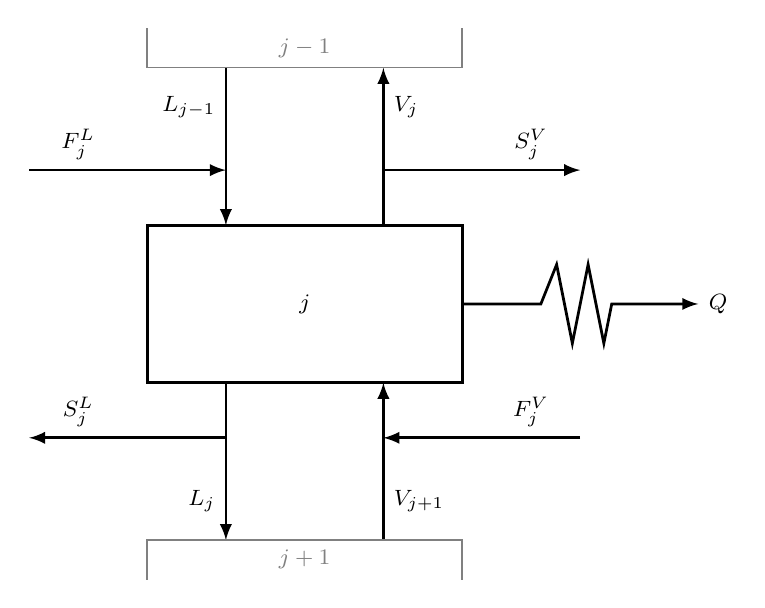
\begin{tikzpicture}[arrow/.style={line width=1pt,->,>=latex}]
	\draw [line width=1pt] (-2,1) rectangle (2,-1) node at (0,0) {\footnotesize $j$};
	\draw [arrow] (-1,3) -- (-1,1) node [pos=0.25, left] {\footnotesize $L_{j-1}$};
 	\draw [arrow] (-3.5,1.7) -- (-1,1.7) node [pos=0.25, above] {\footnotesize $F^L_{j}$};
 	\draw [arrow] (1,1) -- (1,3) node [pos=0.75, right] {\footnotesize $V_{j}$};
 	\draw [arrow] (1,1.7) -- (3.5,1.7) node [pos=0.75, above] {\footnotesize $S^V_{j}$};
 	\draw [arrow] (-1,-1) -- (-1,-3) node [pos=0.75, left] {\footnotesize $L_{j}$};
 	\draw [arrow] (-1,-1.7) -- (-3.5,-1.7) node [pos=0.75, above] {\footnotesize $S^L_{j}$};
	\draw [arrow] (1,-3) -- (1,-1) node [pos=0.25, right] {\footnotesize $V_{j+1}$};
	\draw [arrow] (3.5,-1.7) -- (1,-1.7) node [pos=0.25, above] {\footnotesize $F^V_{j}$};
	\draw [arrow] (2,0) -- (3,0) -- (3.2,0.5) -- (3.4,-0.5) -- (3.6,0.5) -- (3.8,-0.5) -- (3.9,0) -- (5,0,0) node [pos=1, right] {\footnotesize $Q$} ;
    \draw [line width=0.5pt,gray] (-2,-3.5) -- (-2,-3) -- (2,-3) node [pos=0.5, below] {\footnotesize $j+1$} -- (2,-3.5) ; 
    \draw [line width=0.5pt,gray] (-2,3.5) -- (-2,3) -- (2,3) node [pos=0.5, above] {\footnotesize $j-1$} -- (2,3.5) ;
\end{tikzpicture}

                \caption{stage super structure.}
                \label{fig:col_stage_super}
            \end{subfigure}
            %\label{fig:col_super_structs}
            \caption{superstructures for column and column stages.}
        \end{figure}
        \todo{add side draws to column super structure}

        The starting point for the model development is a single separation stage within the
        column with all possible material and energy streams entering and leaving the stage. \Figref{fig:col_super}
        shows the superstructure to be used for the complete column, while \figref{fig:col_stage_super} shows a super
        structure for a single separation stage.

        As mentioned before the governing equations for a distillation column are known as MESH equations. The acronym
        MESH stands for material, equilibrium, summation and enthalpy (often represented by the symbol $H$).
        If not stated otherwise, all equations presented in this section apply to all separation stages. In order
        to improve readability the indices denoting a stage are sometimes omitted, if not essential for the meaning of
        a given equation. throughout the description of the models and the thesis the number of stages in a column section
        will be denoted by $n_S$, while $n_C$, $n_F$, $n_{SV}$ and $n_{SL}$ represent the total number of components,
        feeds, vapour and liquid side draws respectively.

        \ncr{n_S}{number of column stages}{-}
        \ncr{n_C}{number of components}{-}
        \ncr{n_F}{number of feeds}{-}
        \ncr{n_{SV}}{number of vapour side-draws}{-}
        \ncr{n_{SL}}{number of liquid side-draws}{-}

        \paragraph{Material balances} in their most general form for an inner column stage can be written as
        \Eqml{eq:col:CompBalance}{
    		0 = \left(V_j + S_j^V\right) \cdot y_{i,j} + \left(L_j + S_j^L\right) \cdot x_{i,j}
                - V_{j+1} \cdot y_{i,j+1} - L_{j-1} \cdot x_{i,j-1} - F_j \cdot z_{i,j}, \\ \eqanncs.
    	}%
        \ncr{V_j}{molar vapour flowrate form stage $j$}{\mols}
        \ncr{L_j}{molar liquid flowrate form stage $j$}{\mols}
        \ncr{y_{ij}}{vapour mole fraction of component $i$ on stage $j$}{-}
        \ncr{x_{ij}}{liquid mole fraction of component $i$ on stage $j$}{-}
        \ncr{S^L_j}{molar liquid side-draw flowrate form stage $j$}{\mols}
        \ncr{S^V_j}{molar vapour side-draw flowrate form stage $j$}{\mols}
        \ncr{F_j}{feed molar flowrate to stage $j$}{\mols}
        \ncr{z^L_{ij}}{feed mole fraction to stage $j$}{-}
        A certain amount of the liquid or vapour leaving a stage can be withdrawn from the column by means
        of the vapour $S^V_j$ and liquid $S^L_j$ side draw streams. During model development it occurred, that
        when a specification was made on given side-draw, convergence was sometimes hindered. This behaviour
        could be improved by specifying a dimensionless side-draw,
        %
        \Eq{eq:val:vap:strip}{
            s_j^V = \frac{S_j^V}{V_j}, \eqanns, \\
            s_j^L = \frac{S_j^L}{V_j}, \eqanns,
        }%
        \ncr{s^V_j}{dimensionless vapour side-draw from stage $j$}{-}
        \ncr{s^L_j}{dimensionless liquid side-draw from stage $j$}{-}
        %
        rather than an actual stream. Although this technically introduces further non-linearities
        into the material balances. As it is difficult, to guess the dimensionless side draw
        for a desired side draw flowrate, the specification can be replaced by a specification
        on the flowrate, once model initialization has been achieved.

        By considering these dimensionless side-draws the material balance can be rewritten as
        \Eqml{eq:col:CompBalance}{
    		0 = \left(1 + s_j^V\right) \cdot V_j \cdot y_{i,j} + \left(1 + s_j^L\right)
                \cdot L_j \cdot x_{i,j} - V_{j+1} \cdot y_{i,j+1} - L_{j-1} \cdot x_{i,j-1}
                - F_j \cdot z_{i,j}, \\ \eqanncs.
    	}%
        %
        As the model is also to be used for optimization of structural decisions, further extensions are necessary.
        To accommodate that need, new variables are introduced. Particularly split variables $\zeta$ as employed
        by \cite{Dunnebier.1999} are introduced for feeds, vapour and liquid side draws and the reflux location.
        As the feeds are and side draws are to be fed or taken from a single stage, the split variables must assume
        integer values of either one or zero. Furthermore are those decisions \emph{exclusive or} decisions, hence
        \Eq{eq:col:feedsplit}{
            1 =  \sum \zeta.
        }%

        In order to optimize the number of stages several superstructures are possible. One can
        optimize the reboiler reflux location and condenser reflux location or each single one
        along with the feed and side draw locations. The stage number is then changed as all stages
        between condenser or reboiler reflux are effectively rendered inactive. The solution of
        the mass and energy balances for each inactive stage becomes trivial as only one single
        vapour or liquid stream enters and exits the stage.

        While the choice if condenser and or reboiler
        reflux is optimized is somewhat arbitrary some studies have shown \cite{Grossmann.2005} that
        the strategy of optimizing only feed location and reboiler reflux location possesses some
        numerical advantages in terms of performance of the solution algorithm. However this observation
        might be specific to the particular solver used. Furthermore, as will be seen later, there are
        certain situations where optimizing either reboiler or condenser reflux is beneficial in terms of
        problem formulation. The developed model therefore offers capabilities to choose, whether the top
        or bottom reflux is variable. Either reflux will be represented by the generic variable $R$.

        With the newly introduced split variables for the feed $\zeta^F_{ij}$
        as well as the reboiler reflux $\zeta^R_j$ and the liquid $\zeta^{SL}_{ij}$ and vapour $\zeta^{SV}_{ij}$
        side draws, the material balances can be written as
        \Eqml{eq:col:CompBalance_opt}{
    		0 = \left(1 + s_j^V\right) \cdot V_j \cdot y_{i,j} + \left(1 + s_j^L\right)
                \cdot L_j \cdot x_{i,j} - V_{j+1} \cdot y_{i,j+1} \\ \hfill - L_{j-1} \cdot x_{i,j-1}
                - \sum_{k=1}^{n_F} \zeta^F_{kj} \cdot F_j \cdot z_{i,j} - \zeta^R_j \cdot R \cdot z_{R}, \hfill%
                \\ \eqannote{i = 1 \dots C, \quad j = 1 \dots n_S, \quad k = 1 \dots n_F}.
    	}%
        \ncg{\zeta^{F}_{ij}}{splitting variable for feed $i$ on stage $j$}{-}
        \ncg{\zeta^{SV}_{ij}}{splitting variable for vapour side draw $i$ on stage $j$}{-}
        \ncg{\zeta^{SL}_{ij}}{splitting variable for liquid side draw $i$ on stage $j$}{-}
        \ncg{\zeta^{R}_{j}}{splitting variable for reflux on stage $j$}{-}
        %
        Furthermore to be able to optimize side draws, the stripping factors have to be reformulated
        accordingly
        \Eq{eq:val:vap:strip_opt}{
            s_j^V = \frac{\sum_{i=1}^{n_{SV}} \zeta^{SV}_{ij} S_j^V}{V_j}, \eqannote{j = 1 \dots n_S, \quad i = 1 \dots n_{SV}},
        }%
        \Eq{eq:val:liq:strip_opt}{
            s_j^L = \frac{\sum_{i=1}^{n_{SL}} \zeta^{SL}_{ij} S_j^L}{L_j}, \eqannote{j = 1 \dots n_S, \quad i = 1 \dots n_{SL}}.
        }%
        %
        \paragraph{Equilibrium} between a vapour and liquid ia achieved when the chemical potentials for each
        component in both pases are equal. This is commonly expressed by a equilibrium $K_i$ constant. With
        that the equilibrium equation can be written as
        \Eq{eq:col:Kxy}{
            y_{i}^{eq} = K_{i} \cdot x_{i}, \eqannc.
    	}%
        \ncr{K_{ij}}{equilibrium constant of component $i$ on stage $j$}{-}
        \ncr{y_{i}^{eq}}{equilibrium vapour concentration of component $i$ on stage $j$}{\frac{mol}{mol}}
        %
        The requirement for equal chemical potentials can be expressed in terms of the vapour $f_i^V$
        and liquid $f_i^L$ fugacities \cite{AndreasPfennig.2003}.
        \Eq{eq:col:fug}{
            f_i^V = f_i^L, \eqannc.
    	}%
        \ncr{f_i^V}{vapour fugacity}{-}
        \ncr{f_i^L}{liquid fugacity}{-}
        %
        These fugacities are calculated from the liquid activity coefficients $\gamma_i$,
        the pointing factor $F_{Pi}$, the reference vapour fugacity coefficient $\varphi_i$,
        the component saturation pressure $p^S_i$ as well as the system pressure $p$ along
        with the vapour and liquid molar fractions
        \Eq{eq:col:fug_ext}{
            \gamma_i \, F_{Pi} \, \varphi^0_i \, p^S_i \, x_i = \varphi_i \, p \, y_i, \eqannc.
    	}%
        \ncg{\gamma_i}{liquid activity coefficient of component $i$}{-}
        \ncg{\varphi^0_i}{reference vapour fugacity coefficient of component $i$}{-}
        \ncg{\varphi_i}{vapour fugacity coefficient of component $i$}{-}
        \ncr{p^S_i}{vapour pressure of component $i$}{Pa}
        \ncr{p}{system pressure}{Pa}
        \ncr{F_{Pi}}{compressibility factor of component $i$}{-}
        %
        After simple rearrangement \eqref{eq:col:fug_ext} an expression for the equilibrium ratios
        can be derived
        \Eq{eq:col:fug_ext}{
            y_i^{eq} = \underbrace{\frac{\gamma_i \, F_{Pi} \, \varphi^0_i \, p^S_i}{\varphi_i \, p}}_{K_i}
                x_i, \eqannc.
    	}%
        %
        The equations to determine the quantities used when computing the equilibrium ratios are by
        themselves functions of temperature, pressure, and vapour as well as liquid molar fractions.
        They are further discussed in \secref{sec:peng-rob}. It therefore becomes evident that the
        equilibrium ratios are a major source for the non-linearities in the presented model.

        When simulating a distillation process one might consider only equilibrium stages. This however
        will in most cases not reflect the true behaviour of a real stage as the time a vapour and
        liquid phase are in contact might not suffice to achieve equilibrium conditions. This can be
        accounted for by introduction of Murphee tray efficiencies \cite{Henley.op.2011}
        \Eq{eq:ss:murphee}{
            \eta^{eq}_{ij} = \frac{y_{ij} - y_{ij+1}}{y_{ij}^{eq} - y_{ij+1}}, \eqanncs.
        }
        %
        While several models to approximate these efficiencies have been investigated, their predictions are
        most often rather poor \cite{Coulson.1999} and their evaluation rather complex. Furthermore as indicated
        in the formula they might differ for different species involved. For the scope of this model however
        they are not computed separately, but rather supplied and assumed constant for all stages and components.

        \paragraph{Enthalpy balances} are again written considering the previously defined stripping factors
        and splitting variables
    	\Eqml{eq:col:EnergyBalance}{
    		0 = \left(1 + s_j^V\right) \cdot V_j \cdot h^V_{j} + \left(1 + s_j^L\right)
                \cdot L_j \cdot h^L_{j} - V_{j+1} \cdot h^V_{j+1} \\ \hfill - L_{j-1} \cdot h^L_{j-1}
                - \sum_{k=1}^{n_F} \zeta^F_{kj} \cdot F_k \cdot h^{F}_{j} - \zeta^R_j \cdot H_R - Q_j, \hfill
                \\ \eqannote{i = 1 \dots n_C, \quad j = 1 \dots n_S, \quad k = 1 \dots n_F}.
    	}%
        \ncr{h^V_j}{molar vapour enthalpy on stage $j$}{\molenth}
        \ncr{h^L_j}{molar liquid enthalpy on stage $j$}{\molenth}
        \ncr{h^{F}_j}{molar liquid feed enthalpy to stage $j$}{\molenth}
        \ncr{H^{R}}{reflux enthalpy stream}{\molenth}
        %
        \paragraph{Condenser and reboiler} are modeled more or less as regular column stages. However
        they possess certain specialties that are explicitly considered in the column model. For one it is assumed
        that no feeds enter the condenser stage. Furthermore no vapour side stream is drawn from the condenser as well as
        no liquid side stream from the reboiler.

        \begin{figure}
            \centering
            \begin{subfigure}{0.45\textwidth}
                \centering
                \begin{tikzpicture}[scale=0.7]
	\draw [line width=1pt] (-2,1) rectangle (2,-1) node at (0,0) {\footnotesize $1$};
 	\draw [arrow] (1,1) -- (1,3) node [pos=0.75, right] {\footnotesize $V_{1}$};
 	\draw [arrow] (-1,-1) -- (-1,-3) node [pos=0.75, left] {\footnotesize $L_{1}$};
 	\draw [arrow] (-1,-1.7) -- (-3.5,-1.7) node [pos=0.75, above] {\footnotesize $S^L_{1}$};
	\draw [arrow] (1,-3) -- (1,-1) node [pos=0.25, right] {\footnotesize $V_{2}$};
	\draw [arrow] (2,0) -- (3,0) -- (3.2,0.5) -- (3.4,-0.5) -- (3.6,0.5) -- (3.8,-0.5) -- (3.9,0) -- (5,0,0) node [pos=1, right] {\footnotesize $Q^c$} ;
    \draw [line width=0.5pt,gray] (-2,-3.5) -- (-2,-3) -- (2,-3) node [pos=0.5, below] {\footnotesize $2$} -- (2,-3.5) ;
\end{tikzpicture}

                \caption{condenser stage.}
                \label{fig:col_condenser}
            \end{subfigure}
            \begin{subfigure}{0.45\textwidth}
                \centering
                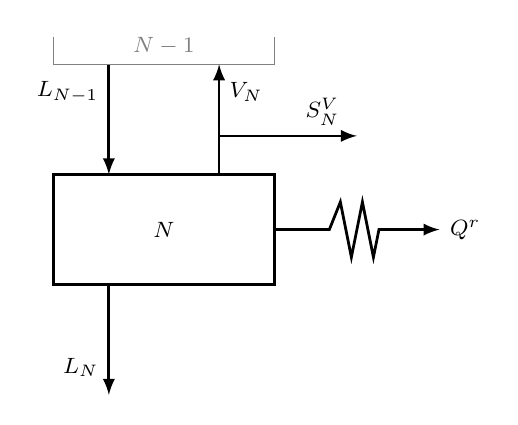
\begin{tikzpicture}[arrow/.style={line width=1pt,->,>=latex},scale=0.7]
	\draw [line width=1pt] (-2,1) rectangle (2,-1) node at (0,0) {\footnotesize $N$};
	\draw [arrow] (-1,3) -- (-1,1) node [pos=0.25, left] {\footnotesize $L_{N-1}$};
 	\draw [arrow] (1,1) -- (1,3) node [pos=0.75, right] {\footnotesize $V_{N}$};
 	\draw [arrow] (1,1.7) -- (3.5,1.7) node [pos=0.75, above] {\footnotesize $S^V_{N}$};
 	\draw [arrow] (-1,-1) -- (-1,-3) node [pos=0.75, left] {\footnotesize $L_{N}$};
	\draw [arrow] (2,0) -- (3,0) -- (3.2,0.5) -- (3.4,-0.5) -- (3.6,0.5) -- (3.8,-0.5) -- (3.9,0) -- (5,0,0) node [pos=1, right] {\footnotesize $Q^r$} ; 
    \draw [line width=0.5pt,gray] (-2,3.5) -- (-2,3) -- (2,3) node [pos=0.5, above] {\footnotesize $N-1$} -- (2,3.5) ;
\end{tikzpicture}

                \caption{reboiler stage.}
                \label{fig:col_reboiler}
            \end{subfigure}
        \end{figure}

        Additionally the condenser stage needs to examined a little further. In terms of operations
        several assumptions can be made for the condenser. In general one can distinguish a total,
        partial vapour and partial vapour liquid condenser. For the total condenser all vapour that
        enters the respective stage is condensed and only liquid product is drawn. The partial vapour
        condenser condenses only the vapour the which is to be fed back into
        the column and all product that is drawn is gaseous. The partial vapour liquid condenser
        denotes the most general case, where part of the incoming vapour is condensed and product
        is drawn from the vapour and liquid phase. The most important thing to consider in these
        different cases is, that while in both partial condensers a vapour liquid equilibrium takes
        place. Due to the absence of vapour the same does not hold for the total condenser. To accommodate
        that fact the MESH equations have to be adjusted \cite{Naphtali.1971}. While the material and energy
        balances remain unchanged the equilibrium equations have to be altered. First the vapour and
        liquid compositions are set equal for all but one component
        \Eq{eq:col:total}{
            x_{i1} = y_{i1} \eqannote{i = 1 \dots C-1},
        }%
        and the condenser temperature is determined by the bubble point equation
        \Eq{eq:col:bub}{
            1 = \sum_i K_{i1}(T_1, p_1,x_1,y_1) \cdot x_{i1} \eqannc.
        }%
        %
        When implementing the model in a process simulator it is sensible to consider, that due to
        the limited accuracy of computers the omitted component in \eqref{eq:col:total} needs to be
        a non-trace component in the condenser stage. The implemented model therefore has to specify
        such a component when a total condenser is chosen to avoid numerical difficulties.

        In practice it is highly unlikely, that the exact amount of energy required to condensate all
        liquid will be drawn from the condenser. More likely, if all vapour is condensed, slightly more
        energy will be withdrawn and sub-cooled liquid will leave the condenser. Therefore
        the model includes the possibility to specify a degree of sub-cooling $T^{sub}$ which will be
        considered when calculating bubble point temperature
        %
        \Eq{eq:col:bub}{
            1 = \sum_i K_{i1}(T_1 + T^{sub}, p_1,x_1,y_1) \cdot x_{i1} \eqannc.
        }%
        \ncr{T^{sub}}{sub-cooling temperature}{K}
        %
        \paragraph{Pressure} along the entire column is often specified in the steady-state case.
        However as it is inconvenient and unpractical to specify a pressure for each stage one might either specify
        a pressure at the top and bottom stage and assume a uniform pressure profile along the column, or
        specify either top $p_1$ or bottom pressure $p_N$ along with a total pressure drop $\Delta p$,
        or a stage-wise one $\Delta p_{stage}$. However the issue is further complicated if one considers the
        case of optimization for number of trays. In that case several trays will become inactive. For those
        trays the mass and energy balances become trivial, as only liquid enters and exits these trays.
        (For the case employed here, where the reboiler reflux is being optimized). This also means,
        that from the last active tray down to the reboiler -- if present -- there should be a uniform
        profile. It is important to note, that if a uniform pressure profile from the lowest active stage
        downward is not enforced, the solver will have to compensate for slight changes in the equilibrium
        due to pressure variations with minimal vapour flow-rates. This is very undesirable, as it might to
        lead to severe problems in the solver, or the calculation of other properties, dependent on these values.
        To account for this issue, the reboiler reflux split be employed to deactivate the pressure drop
        \Eq{}{
            p_i = p_{j-1} + \left(1 - \sum_{k=1}^{j-1} \zeta^R_k \right) \cdot \Delta p_{j-1} \eqanns.
        }
        \ncr{\Delta p}{pressure drop over entire column}{Pa}
        \ncr{\Delta p_{stage}}{stage-wise pressure drop}{Pa}
        %
        \todo{adjust pressure equation to accommodate variable top and bottom tray}
        As an alternative to specifying the pressure, one might consider calculating the pressure drop
        form (semi)-empirical models. There a numerous correlations for different types of column internals.
        These correlations become particularly important if column dynamics are to be considered, as they
        form the connection between holdups and flow-rates within the column. Two different pressure drop models
        have been implemented, one for trayed columns and another one for structured packings. As they are closely
        tied to dynamics, they will be discussed in more detail in \secref{chp:dynamics}.

    \subsubsection{Specifications \& initialization}
    \label{sec:mathpro:steady:specinit}
        \todo{section superfluous? init procedure describen in impl sec...}
        The equation systems presented above is comprised of $n_S n_C$ component balances and equilibrium
        equations, $2n_S$ summation equations and $n_S$ energy balances. This gives a total of $n_S (2n_C + 3)$
        equations. On the other hand there are $n_S$ temperatures and pressures, $2n_S$ molar flow rates,
        $n_S$ energy streams, and $n_S n_C$ vapour as well as and liquid concentrations. Additionally the feed flow rates
        compositions and temperatures and the side draw split fractions or flow rates appear as variables. The
        feeds and side draws would usually be specified, which leaves a total of $n_S (2n_C + 5)$ variables.

        The pressure profile of a distillation column is usually specified.
        In terms of unit operations this pressure drop is of high significance,
        as many columns can only be feasibly operated, if the pressure drop does not exceed certain
        limits. In case of the ASU the production of Argon only became feasible as structured
        packings, which display a very low pressure drop, became available. This is due to the large
        number of theoretical stages required to attain the desired Argon purities.

        The energies $Q_i$ denote addition heaters or cooler on the respective stages. For all
        intermediate stages these values would be specified as well. If all energies are
        specified, that would -- along with the pressure profile -- sum up to $2 n_S$ specifications,
        which leaves $n_S (2n_C + 3)$ unknowns. As the number of equations and unknowns are the equal,
        this system is then well specified.

        In practice it is often challenging to correctly guess the condenser and reboiler heat loads in
        advance. This is especially true since they have a tremendous impact on the overall performance
        of the column. Hence it is often desirable to supply other specifications than the respective
        heat loads. To allow for such specification so called discrepancy functions can be introduced
        \cite{Henley.op.2011}, which replace the energy balance for the condenser and / or reboiler stage.

        One common specification is the so called reflux ratio $\nu^D = \frac{L_1}{V_1 + S_1^L}$ for
        the condenser, or the boil-up ratio $\nu^R = \frac{L_N}{V_N}$ for the reboiler.
        They are defined as the ratio of the molar flowrate sent back into the column over the
        product flowrate which leaves the column. For the reboiler this denotes a liquid stream,
        while for the condenser the product can be gaseous and liquid. Specifying this leads to
        \Eq{eq:reflux}{
            0 & = L_1 - \nu^D \cdot (V_1 + S_1^L), \\
            0 & = V_N - \nu^R \cdot L_N,
        }
        \ncg{\nu^R}{boliup ratio}{-}
        \ncg{\nu^D}{reflux ratio}{-}
        as discrepancy functions. I addition to that further specifications are conceivable. Most
        commonly distillate ($D$) or bottoms ($B$) flow rates, purities, component flow rates ($d_i, b_i$)
        or temperatures. The corresponding discrepancy functions are summarized in \tabref{tab:discrepancy}.

        \begin{table}
            \centering
            \footnotesize
            \begin{tabular}{lll}
	specification & replacement for $H_1$ & replacement for $H_N$ \\ \hline
	reflux or boilup ratio & $0  = L_1 - \nu^D \cdot (V_1 + S_1^L)$ & $0  = V_N - \nu^R \cdot L_N$ \\
	temperature & $0 = T_1 - T_{spec}$ & $0 = T_N - T_{spec}$ \\
	product flowrate & $0 = (V_1 + S_1^L) - D$ & $0 = L_N - B$ \\
	component product flowrate & & $0 = L_N \cdot x_{iN} - b_i$ \\
	mole fraction & $0 = y_{i1} - y_{i,spec}$ & $0 = x_{iN} - x_{ispec}$ \\ \hline
\end{tabular}

            \caption{discrepancy functions for different column specifications.}
            \label{tab:discrepancy}
        \end{table}

        The specifications for the reboiler stage are quite straightforward, in contrast to that,
        different cases for the condenser have to be considered. In the most general case the
        top product can be drawn as vapour and liquid. This case is here called a partial vapour
        liquid condenser. The other cases are a total condenser, where all the vapour entering the
        condenser stage is condensed, and all product is drawn as a liquid stream, as well as
        a partial vapour condenser, where only the reflux is condensed and all product is drawn
        as vapour. As discussed earlier no VLE takes place in the condenser stage, if a total
        condenser is specified, which needs to be accounted for. Both the total and partial
        vapour condensed implicitly include an extra specification since in former case
        the top vapour product flow rate becomes zero and in the latter the top liquid product
        flowrate. Furthermore a specification of the condenser energy is infeasible as well as implicitly
        given for the total condenser. In case of the partial vapour liquid condenser no implicit
        specification is given, which requires an additional specification. In general two
        top specifications are necessary, whereas only one bottom specification is required.
        These top specification can include the condenser duty, any top flowrate, the reflux ratio
        as well as a newly introduced quantity, the top vapour fraction defined as
        \Eq{}{
            \nu^{vap} = \frac{V_1}{V_1 + S_1^L}.
        }
        \ncg{\nu^{vap}}{condenser vapour fraction}{-}
        %
        As mentioned before the solution of the MESH equations can pose a considerable problem
        to numerical solvers. It is therefore necessary to supply the solver with feasible
        estimates for the involved variables that can be used as an initial guess for
        convergence of the process model. A lot of effort has been spend to formulate robust strategies
        to initialize distillation column models. One of the most prominent is the so called
        Inside-Out algorithm first introduced by Boston and Sullivan \cite{Boston.1974}. Within this
        algorithm an inner and outer iterative loop are employed. Within the outer loop approximate
        parameters for simplified models of phase equilibrium and enthalpy are computed by rigorous
        thermodynamic models and guesses for stage temperatures and concentrations. Within the
        inner loop new stage temperatures and concentrations are attained by solving the MESH equations
        using the simplified thermodynamic models. Once the inner loop converges the simplified
        model parameters are updated within the outer loop by means of the newly calculated
        temperatures and concentrations. This algorithm converges in many cases even for very poor initial
        guesses and has been extended to handle complex columns with side-draws and even reactive
        distillation \cite{Boston.}. It is still in use in the process simulator \aspen.
        However as it is used within an modular algorithmic environment it is not applicable
        to equation based simulators such as \gproms.

        More recently other approaches have been published to attain improved initial guesses.
        Fletcher and Morton \cite{Fletcher.2000} proposed the solution of a column model at
        infinite reflux and zero feed flow rate. This leads to a much simplified model which can
        be solved more easily. The computed purities and stage numbers can give valuable insight
        into the process model. As this approach relies on the solution of a simplified model
        and has no algorithmic elements, it can be implemented in equation based process simulators.

        Another strategy that has been successfully applied to zeotropic and azeotropic mixtures
        relies on solving the column model for the limiting case of the adiabatic column \cite{Barttfeld.2002}.
        The adiabatic column in this case is the column with the minimal entropy production in a real column.
        To avoid entropy production all streams that come in contact must be in equilibrium. To achieve this
        the column would have to employ an infinite number of stages and have an infinite number of
        heat exchangers along its length. The adiabatic column then uses only two heat exchanger in the
        condenser and reboiler stage and assumes a pinch point at the feed stage. \todo{elaborate on adiabatic column}

        Furthermore a much simpler approach has proven adequate for many applications \cite{Henley.op.2011}
        which is also employed as a starting point in this work.
        Therein feed properties are used as initial guesses. First a linear temperature profile form the boiling
        temperature to dew temperature of the combined feed mixture is used to initialize temperatures, whereas a simple flash
        at average column pressure and feed temperature yields a vapour and liquid concentration which is
        used as uniform profile for every column stage. However as the feed might be sub-cooled liquid or
        super-heated vapour, the TP-Flash is replaced by a specified vapour fraction. As vapour fraction
        for the flash initial estimates of the vapour and liquid flow rates at the top and bottom of the
        column are used. The stage-wise molar flow-rates are computed from the constant molal overflow
        assumption, which postulates a constant heat of vaporization and yields therefore uniform
        liquid and vapour flow-rates within a column section. A section in this case is denoted by any
        feed location where the flow-rates change due to the added feed. In the feed stages a super heated
        or sub-cooled feed is also considered by means of an extended vapour fraction
        \Eq{}{
            q^F = \frac{h^F - h^L}{h^V - h^L}.
        }
        %
        While this approach leads to model convergence in many cases, it is not entirely robust.
        While the system considered in this case displays only moderate non-idealities it is highly cupeled.
        Especially the low pressure column (LPC) has multiple feeds and side draws, which leads to non-convergence
        if the aforementioned initialization strategy is employed. However the fact that the system is
        not highly non-ideal can be exploited. Whenever the K-values are not too much dependent on mixture
        composition an intermediate step can be used to refine concentration guesses. The constant molal
        overflow assumption is retained and the equilibrium ratios are computed based on the initial guesses
        from the first stage. The component balance is then reformulated only in terms of liquid component
        flow-rates $l_{ij}$
        %
        \Eqml{eq:init:compbalance}{
            0 = \left((1+s_j^V) \cdot K_{ij} \cdot \frac{V_j}{L_j} + (1+s_j^L) \right) \cdot l_{ij}
                - \frac{V_{j+1}}{L_{j+1}} \cdot K_{ij+1} \cdot l_{ij+1} - l_{ij-1}
                \\ - F_j^V \cdot z^V_{i,j} - F_j^L \cdot z_{i,j}^L, \eqanncs.
        }%
        \ncr{l_{ij}}{liquid molar flowrate of component $i$ from stage $j$}{\mols}
        \ncr{v_{ij}}{vapour molar flowrate of component $i$ from stage $j$}{\mols}
        %
        \eqref{eq:init:compbalance} is linear in the liquid component flow rates. Furthermore vapour component
        flow rates are substituted in the linear component balance and can be computed by
        %
        \Eq{eq:init:vapflow}{
            v_{ij} =  K_{ij} \cdot \frac{V_j}{L_j} \cdot l_{ij} \eqanncs.
        }%
        %
        On of the reasons \eqref{eq:init:compbalance} is formulated in terms of component flow rates rather
        than molar fractions, is that the molar fraction computed in that manner would not be normalized. If
        the mole fractions are computed from the component flow rates normalization is implicitly given
        %
        \Eq{eq:init:liqmolefrac}{
            x_{ij} = \frac{l_{ij}}{\sum_k^C l_{kj}} \eqanncs,
        }%
        \Eq{eq:init:vapmolefrac}{
            y_{ij} = \frac{v_{ij}}{\sum_k^C v_{kj}} \eqanncs.
        }%
        %
        The total molar flow rates used in \eqref{eq:init:compbalance} are computed by solving
        stage-wise total mass balances under the constant molal overflow assumption. This assumption
        postulates that the heat of vaporization is independent of system composition.
        Therefore always the same amount of liquid enters and leaves a given stage
    	\Eq{eq:col:cmo}{
    		0 = L_j + S_j^L - L_{j-1} - (1 - q^F) \cdot F_j \eqannote{j = 1 \dots n_S}.
    	}%
        \ncr{F_j}{feed to tray $j$}{\frac{mol}{s}}
    	\ncr{S_j^V}{vapour side flow from tray $j$}{\frac{mol}{s}}
    	\ncr{S_j^L}{liquid side flow from tray $j$}{\frac{mol}{s}}
    	\ncr{V_j}{vapour flow from tray $j$}{\frac{mol}{s}}
    	\ncr{L_j}{liquid flow from tray $j$}{\frac{mol}{s}}
        %
        The vapour total flow rates are then computed from the total mass balances
        \Eq{eq:col:MassBalance}{
    		0 = L_j + S_j^L + V_j + S_j^V - L_{j-1} - V_{j+1} - F_j^,
                \eqannote{j = 1 \dots n_S}.
    	}%
        %
        As no energy balances are included at this stage, the condenser and reboiler stage
        are characterized by the reflux ($\nu^c = \frac{V_1}{L_1}$) or boilup ratio
        ($\nu^r = \frac{V_N}{L_N}$) respectively. This leads to
        \Eq{eq:boilup}{
            0 = V_1 - \nu^c \cdot L_1, \\
            0 = L_N - \nu^r \cdot V_N.
        }
        %
        To close the equation system the global mass balance is included
        \Eq{eq:globalmassbalance}{
            0 = V_1 + L_N + \sum_{j=1}^{N} ( S_j^V + S_j^L - F_j),
                \eqannote{j = 1 \dots n_S}.
        }
        %
        \todo{check equations in steady state section!!!}
        For more complex systems more elaborate strategies have been developed, which essentially try
        to incorporate some of the principals from the inside out algorithm into an equation based
        environment. The process simulator \gproms allows for definition of standardized initialization
        procedures as well as different model variants that can be solved consecutively. With that strategies
        were developed that proved successful for more complex mixtures and even three phase systems. As
        these strategies are closely linked to the implementation in \gproms and the programm
        capabilities, they will be discussed in \secref{sec:mathpro:implementation}

        Furthermore ist should be noted, that not all specifications are compatible with the initialization
        strategies described above. While this issue has been addressed, it also will be explained in the
        implementation section.

        \paragraph{Example}

        \begin{figure}
            \begin{minipage}{0.25\textwidth}
                \begin{tikzpicture}[scale=0.5]
	\draw [line width=0.5pt,gray] (1,4.8) -- (-1,4.8) node [above,pos=0.5,black,yshift=-1mm] {\footnotesize 1};
    \draw [line width=0.5pt,gray] (1,-4.8) -- (-1,-4.8) node [above,pos=0.5,black,yshift=-1mm] {\footnotesize 69};
    \draw [line width=0.5pt,gray] (1,3.2) -- (-1,3.2) node [above,pos=0.5,black,yshift=-1mm] {\footnotesize 10};
    \draw [line width=0.5pt,gray] (1,1.6) -- (-1,1.6) node [above,pos=0.5,black,yshift=-1mm] {\footnotesize 21};
    \draw [line width=0.5pt,gray] (1,0.0) -- (-1,0.0) node [above,pos=0.5,black,yshift=-1mm] {\footnotesize 28};
    \draw [line width=0.5pt,gray] (1,-3.2) -- (-1,-3.2) node [above,pos=0.5,black,yshift=-1mm] {\footnotesize 55};
	\draw [line width=1pt, rounded corners] (-1.0,-5) -- (-1.0,5) .. controls (-0.8,5.8) and (0.8,5.8) .. (1.0,5) node (a) [inner sep=0cm , pos=0.5] {} -- (1.0,-5) .. controls (0.8,-5.8) and (-0.8,-5.8) .. (-1.0,-5) node (b) [inner sep=0cm , pos=0.5] {} -- cycle ; % column tower
    \draw [arrow] (b) -- (0,-6.2) -- (2.5,-6.2) node [draw, line width=1pt, pos=1, circle, minimum size=1.0cm, fill=white] {} -- (2.5,-4.8) -- (1,-4.8) ; % circle reboiler
    \draw [line width=0.5pt] (4,-6.5) -- (2.2,-6.5) -- (2.6,-6.2) -- (2.2,-5.9) -- (4,-5.9) ; % heater reboiler
	\draw [arrow] (-3.0,4.8) -- (-1,4.8) node [above,pos=0.5,black,yshift=-1mm] {\footnotesize $F_1$} ;
    \draw [arrow] (-3.0,1.6) -- (-1,1.6) node [above,pos=0.5,black,yshift=-1mm] {\footnotesize $F_2$} ;
    \draw [arrow] (-3.0,0.0) -- (-1,0.0) node [above,pos=0.5,black,yshift=-1mm] {\footnotesize $F_3$} ;
    \draw [arrow] (-3.0,-3.2) -- (-1,-3.2) node [above,pos=0.5,black,yshift=-1mm] {\footnotesize $F_4$} ;
    \draw [arrow] (1.0,3.2) -- (3.0,3.2) node [above,pos=0.5,black,yshift=-1mm] {\footnotesize $S_1$} ;
    \draw [arrow] (1.0,-3.2) -- (3,-3.2) node [above,pos=0.5,black,yshift=-1mm] {\footnotesize $S_2$} ;
    \draw [arrow] (2.5,-4.8) -- (4,-4.8) ;
    \node at (1.9,-6.2) {\footnotesize 70} ;
    \draw [arrow] (a) -- (0.0,6.5) -- (3.0,6.5) ;
\end{tikzpicture}

                \caption{example column.}
                \label{fig:lpc_example}
            \end{minipage}
            \begin{minipage}{0.73\textwidth}
                \raisebox{\depth}{\footnotesize\begin{tabular}{C{0.08\textwidth}C{0.15\textwidth}C{0.12\textwidth}C{0.12\textwidth}C{0.12\textwidth}C{0.09\textwidth}C{0.09\textwidth}}
    \multicolumn{7}{c}{feed specifications} \\ \hline
	stream & flow $[\frac{kmol}{hr}]$ & $z_{O_2} [-]$ & $z_{N_2} [-]$ & $z_{Ar} [-]$ & $T [K]$ & $p [bar]$ \\ 
	$F_1$ & 2985.77 & 4.674E-10 & 0.9999 & 6.378E-7 & 79.45 & 1.3 \\
	$F_2$ & 1836.36 & 0.2095 & 0.7812 & 0.0093 & 98.91 & 1.3 \\
	$F_3$ & 7609.06 & 0.2920 & 0.6950 & 0.0130 & 81.88 & 1.3 \\
	$F_4$ & 774.94 & 0.9161 & 5.393E-12 & 8.394E-2 & 92.13 & 1.8 \\ \hline 
    & & & & & & \\
    \multicolumn{7}{c}{column specifications} \\ \hline
    stages & $S_1$ frac & $S_2$ frac & \multicolumn{2}{c}{boilup ratio} & $p^{top}$ & $p^{bot}$ \\
    70 & 10 & 0.15 & \multicolumn{2}{c}{3.5} & 1.2 bar & 1.3 bar \\ \hline
\end{tabular}
}
                \captionof{table}{column specifications.}
                \label{fig:lpc_example}
            \end{minipage}
        \end{figure}

        To illustrate how the initialization procedure works an example has been constructed of
        a rather complex column -- or column section -- with multiple feeds and side draws (\figref{fig:lpc_example}).
        It is taken from an example process of cryogenic air separation. The column in question
        is a column section without an condenser stage and displayed the most difficulties in terms
        of convergence when constructing the process flowsheet.

        In addition to the aforemention initialization strategy, columns with side draws present are handled
        in a slightly different manner. Initially the side draws are disregarded. Then the initialization procedure
        is carried out. Once the column without side draws has converged, a homotopy approach
        \Eq{eq:homotopy}{
            f(\vec{x}) = (1-\alpha) \cdot f_0(\vec{x}) + \alpha \cdot f_1(\vec{x})
        }
        is employed, where the parameter $\alpha$ is initially set to zero and then gradually moved to a value
        of one. \todo{mention problems and bounded homotopy?} During the initialization homotopies could
        generally be employed to move from one step to another. While in some cases robustness is improved by
        such a strategy, it is always computationally far more expensive then simply jumping between different
        stages.

        For clarity reasons the different steps of the initializations procedure a repeated in a tabular manner

        \begin{enumerate}
            \item \cpitemize{
                \item linear temperature profile between dew ($T^{dew}$) and bubble point temperature ($T^{bub}$)
                    of mixed feed.
                \item linear profile between feed flash vapour and liquid compositions for liquid stage
                    compositions.
                \item constant profile for vapour compositions.
                \item molar flow rates from constant molar overflow model.
                \item side draw flow rates set to zero.
            }
            \item \cpitemize{
                \item total molar flow rates form constant molar overflow model.
                \item simplified equilibrium ratios from initial liquid mole fractions and linear
                    temperature profile.
                \item liquid and vapour mole fractions from linearized mass balances.
            }
            \item rigorous solution of MESH equations with side draws still set to zero.
            \item homotopic approach to MESH equations with side draws considered.
        \end{enumerate}

        \ncr{T^{dew}}{dew point temperature}{K}
        \ncr{T^{bub}}{bubble point temperature}{K}

        The resulting profiles for oxygen and nitrogen concentrations in the example column can be seen
        in \figref{fig:lpc_example_o2} and \figref{fig:lpc_example_n2}.

        \begin{figure}
            \scriptsize
            \hspace{0.01\textwidth}
            \begin{subfigure}{0.45\textwidth}
                % GNUPLOT: LaTeX picture with Postscript
\begingroup
  \makeatletter
  \providecommand\color[2][]{%
    \GenericError{(gnuplot) \space\space\space\@spaces}{%
      Package color not loaded in conjunction with
      terminal option `colourtext'%
    }{See the gnuplot documentation for explanation.%
    }{Either use 'blacktext' in gnuplot or load the package
      color.sty in LaTeX.}%
    \renewcommand\color[2][]{}%
  }%
  \providecommand\includegraphics[2][]{%
    \GenericError{(gnuplot) \space\space\space\@spaces}{%
      Package graphicx or graphics not loaded%
    }{See the gnuplot documentation for explanation.%
    }{The gnuplot epslatex terminal needs graphicx.sty or graphics.sty.}%
    \renewcommand\includegraphics[2][]{}%
  }%
  \providecommand\rotatebox[2]{#2}%
  \@ifundefined{ifGPcolor}{%
    \newif\ifGPcolor
    \GPcolortrue
  }{}%
  \@ifundefined{ifGPblacktext}{%
    \newif\ifGPblacktext
    \GPblacktexttrue
  }{}%
  % define a \g@addto@macro without @ in the name:
  \let\gplgaddtomacro\g@addto@macro
  % define empty templates for all commands taking text:
  \gdef\gplbacktext{}%
  \gdef\gplfronttext{}%
  \makeatother
  \ifGPblacktext
    % no textcolor at all
    \def\colorrgb#1{}%
    \def\colorgray#1{}%
  \else
    % gray or color?
    \ifGPcolor
      \def\colorrgb#1{\color[rgb]{#1}}%
      \def\colorgray#1{\color[gray]{#1}}%
      \expandafter\def\csname LTw\endcsname{\color{white}}%
      \expandafter\def\csname LTb\endcsname{\color{black}}%
      \expandafter\def\csname LTa\endcsname{\color{black}}%
      \expandafter\def\csname LT0\endcsname{\color[rgb]{1,0,0}}%
      \expandafter\def\csname LT1\endcsname{\color[rgb]{0,1,0}}%
      \expandafter\def\csname LT2\endcsname{\color[rgb]{0,0,1}}%
      \expandafter\def\csname LT3\endcsname{\color[rgb]{1,0,1}}%
      \expandafter\def\csname LT4\endcsname{\color[rgb]{0,1,1}}%
      \expandafter\def\csname LT5\endcsname{\color[rgb]{1,1,0}}%
      \expandafter\def\csname LT6\endcsname{\color[rgb]{0,0,0}}%
      \expandafter\def\csname LT7\endcsname{\color[rgb]{1,0.3,0}}%
      \expandafter\def\csname LT8\endcsname{\color[rgb]{0.5,0.5,0.5}}%
    \else
      % gray
      \def\colorrgb#1{\color{black}}%
      \def\colorgray#1{\color[gray]{#1}}%
      \expandafter\def\csname LTw\endcsname{\color{white}}%
      \expandafter\def\csname LTb\endcsname{\color{black}}%
      \expandafter\def\csname LTa\endcsname{\color{black}}%
      \expandafter\def\csname LT0\endcsname{\color{black}}%
      \expandafter\def\csname LT1\endcsname{\color{black}}%
      \expandafter\def\csname LT2\endcsname{\color{black}}%
      \expandafter\def\csname LT3\endcsname{\color{black}}%
      \expandafter\def\csname LT4\endcsname{\color{black}}%
      \expandafter\def\csname LT5\endcsname{\color{black}}%
      \expandafter\def\csname LT6\endcsname{\color{black}}%
      \expandafter\def\csname LT7\endcsname{\color{black}}%
      \expandafter\def\csname LT8\endcsname{\color{black}}%
    \fi
  \fi
  \setlength{\unitlength}{0.0500bp}%
  \begin{picture}(4762.00,2834.00)%
    \gplgaddtomacro\gplbacktext{%
      \csname LTb\endcsname%
      \put(758,512){\makebox(0,0)[r]{\strut{} 0.0}}%
      \put(758,938){\makebox(0,0)[r]{\strut{} 0.2}}%
      \put(758,1364){\makebox(0,0)[r]{\strut{} 0.4}}%
      \put(758,1789){\makebox(0,0)[r]{\strut{} 0.6}}%
      \put(758,2215){\makebox(0,0)[r]{\strut{} 0.8}}%
      \put(758,2641){\makebox(0,0)[r]{\strut{} 1.0}}%
      \put(1317,352){\makebox(0,0){\strut{} 10}}%
      \put(1831,352){\makebox(0,0){\strut{} 20}}%
      \put(2346,352){\makebox(0,0){\strut{} 30}}%
      \put(2860,352){\makebox(0,0){\strut{} 40}}%
      \put(3374,352){\makebox(0,0){\strut{} 50}}%
      \put(3889,352){\makebox(0,0){\strut{} 60}}%
      \put(4403,352){\makebox(0,0){\strut{} 70}}%
      \put(198,1576){\rotatebox{-270}{\makebox(0,0){\strut{}mole fraction $[-]$}}}%
      \put(2628,112){\makebox(0,0){\strut{}stage number $[\#]$}}%
    }%
    \gplgaddtomacro\gplfronttext{%
      \csname LTb\endcsname%
      \put(3908,1135){\makebox(0,0)[r]{\strut{}step 1}}%
      \csname LTb\endcsname%
      \put(3908,975){\makebox(0,0)[r]{\strut{}step 2}}%
      \csname LTb\endcsname%
      \put(3908,815){\makebox(0,0)[r]{\strut{}step 3}}%
      \csname LTb\endcsname%
      \put(3908,655){\makebox(0,0)[r]{\strut{}conv}}%
    }%
    \gplbacktext
    \put(0,0){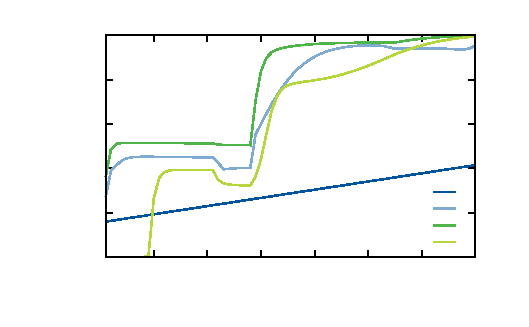
\includegraphics{GNUPlot/LPC_init_o2}}%
    \gplfronttext
  \end{picture}%
\endgroup

                \caption{oxygen concentration profiles.}
                \label{fig:lpc_example_o2}
            \end{subfigure}
            \hfill
            \begin{subfigure}{0.45\textwidth}
                % GNUPLOT: LaTeX picture with Postscript
\begingroup
  \makeatletter
  \providecommand\color[2][]{%
    \GenericError{(gnuplot) \space\space\space\@spaces}{%
      Package color not loaded in conjunction with
      terminal option `colourtext'%
    }{See the gnuplot documentation for explanation.%
    }{Either use 'blacktext' in gnuplot or load the package
      color.sty in LaTeX.}%
    \renewcommand\color[2][]{}%
  }%
  \providecommand\includegraphics[2][]{%
    \GenericError{(gnuplot) \space\space\space\@spaces}{%
      Package graphicx or graphics not loaded%
    }{See the gnuplot documentation for explanation.%
    }{The gnuplot epslatex terminal needs graphicx.sty or graphics.sty.}%
    \renewcommand\includegraphics[2][]{}%
  }%
  \providecommand\rotatebox[2]{#2}%
  \@ifundefined{ifGPcolor}{%
    \newif\ifGPcolor
    \GPcolortrue
  }{}%
  \@ifundefined{ifGPblacktext}{%
    \newif\ifGPblacktext
    \GPblacktexttrue
  }{}%
  % define a \g@addto@macro without @ in the name:
  \let\gplgaddtomacro\g@addto@macro
  % define empty templates for all commands taking text:
  \gdef\gplbacktext{}%
  \gdef\gplfronttext{}%
  \makeatother
  \ifGPblacktext
    % no textcolor at all
    \def\colorrgb#1{}%
    \def\colorgray#1{}%
  \else
    % gray or color?
    \ifGPcolor
      \def\colorrgb#1{\color[rgb]{#1}}%
      \def\colorgray#1{\color[gray]{#1}}%
      \expandafter\def\csname LTw\endcsname{\color{white}}%
      \expandafter\def\csname LTb\endcsname{\color{black}}%
      \expandafter\def\csname LTa\endcsname{\color{black}}%
      \expandafter\def\csname LT0\endcsname{\color[rgb]{1,0,0}}%
      \expandafter\def\csname LT1\endcsname{\color[rgb]{0,1,0}}%
      \expandafter\def\csname LT2\endcsname{\color[rgb]{0,0,1}}%
      \expandafter\def\csname LT3\endcsname{\color[rgb]{1,0,1}}%
      \expandafter\def\csname LT4\endcsname{\color[rgb]{0,1,1}}%
      \expandafter\def\csname LT5\endcsname{\color[rgb]{1,1,0}}%
      \expandafter\def\csname LT6\endcsname{\color[rgb]{0,0,0}}%
      \expandafter\def\csname LT7\endcsname{\color[rgb]{1,0.3,0}}%
      \expandafter\def\csname LT8\endcsname{\color[rgb]{0.5,0.5,0.5}}%
    \else
      % gray
      \def\colorrgb#1{\color{black}}%
      \def\colorgray#1{\color[gray]{#1}}%
      \expandafter\def\csname LTw\endcsname{\color{white}}%
      \expandafter\def\csname LTb\endcsname{\color{black}}%
      \expandafter\def\csname LTa\endcsname{\color{black}}%
      \expandafter\def\csname LT0\endcsname{\color{black}}%
      \expandafter\def\csname LT1\endcsname{\color{black}}%
      \expandafter\def\csname LT2\endcsname{\color{black}}%
      \expandafter\def\csname LT3\endcsname{\color{black}}%
      \expandafter\def\csname LT4\endcsname{\color{black}}%
      \expandafter\def\csname LT5\endcsname{\color{black}}%
      \expandafter\def\csname LT6\endcsname{\color{black}}%
      \expandafter\def\csname LT7\endcsname{\color{black}}%
      \expandafter\def\csname LT8\endcsname{\color{black}}%
    \fi
  \fi
  \setlength{\unitlength}{0.0500bp}%
  \begin{picture}(4762.00,2834.00)%
    \gplgaddtomacro\gplbacktext{%
      \csname LTb\endcsname%
      \put(758,512){\makebox(0,0)[r]{\strut{} 0.0}}%
      \put(758,938){\makebox(0,0)[r]{\strut{} 0.2}}%
      \put(758,1364){\makebox(0,0)[r]{\strut{} 0.4}}%
      \put(758,1789){\makebox(0,0)[r]{\strut{} 0.6}}%
      \put(758,2215){\makebox(0,0)[r]{\strut{} 0.8}}%
      \put(758,2641){\makebox(0,0)[r]{\strut{} 1.0}}%
      \put(1317,352){\makebox(0,0){\strut{} 10}}%
      \put(1831,352){\makebox(0,0){\strut{} 20}}%
      \put(2346,352){\makebox(0,0){\strut{} 30}}%
      \put(2860,352){\makebox(0,0){\strut{} 40}}%
      \put(3374,352){\makebox(0,0){\strut{} 50}}%
      \put(3889,352){\makebox(0,0){\strut{} 60}}%
      \put(4403,352){\makebox(0,0){\strut{} 70}}%
      \put(198,1576){\rotatebox{-270}{\makebox(0,0){\strut{}mole fraction $[-]$}}}%
      \put(2628,112){\makebox(0,0){\strut{}stage number $[\#]$}}%
    }%
    \gplgaddtomacro\gplfronttext{%
      \csname LTb\endcsname%
      \put(3908,1135){\makebox(0,0)[r]{\strut{}step 1}}%
      \csname LTb\endcsname%
      \put(3908,975){\makebox(0,0)[r]{\strut{}step 2}}%
      \csname LTb\endcsname%
      \put(3908,815){\makebox(0,0)[r]{\strut{}step 3}}%
      \csname LTb\endcsname%
      \put(3908,655){\makebox(0,0)[r]{\strut{}conv}}%
    }%
    \gplbacktext
    \put(0,0){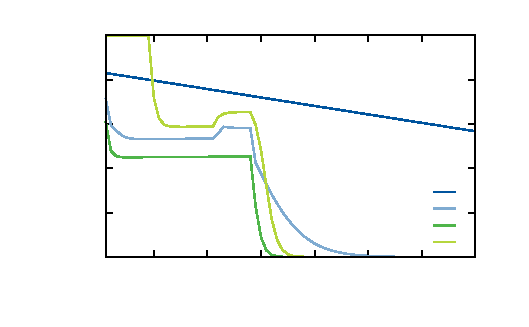
\includegraphics{GNUPlot/LPC_init_n2}}%
    \gplfronttext
  \end{picture}%
\endgroup

                \caption{nitrogen concentration profiles.}
                \label{fig:lpc_example_n2}
            \end{subfigure}
            \hspace{0.01\textwidth}
            \caption{initialization example concentration profiles.}
        \end{figure}



 \subsection{Integrated condenser \& reboiler}
    \label{sec:mathpro:steady:conreb}
        \begin{figure}
            \center
            \begin{tikzpicture}
    \pgfmathsetmacro{\unitwidth}{5} ;
    \pgfmathsetmacro{\unitheight}{3} ;
    \pgfmathsetmacro{\domerad}{0.5*\unitwidth/2} ;
    \pgfmathsetmacro{\lang}{76} ;
    \pgfmathsetmacro{\rang}{180-\lang} ;
    \pgfmathsetmacro{\conheight}{0.7*\unitheight} ;
    \pgfmathsetmacro{\conwidth}{0.45*\unitwidth} ;
    
    \draw [line width=0.5pt,rounded corners] (-0.5*\unitwidth,0) -- ++(0,0.5*\unitheight) .. controls +(\lang:\domerad) and +(\rang:\domerad) .. (0.5*\unitwidth,0.5*\unitheight) node (top) [pos=0.5,inner sep=0] {} -- ++(0,-\unitheight) .. controls +(-\rang:\domerad) and +(-\lang:\domerad) .. (-0.5*\unitwidth,-0.5*\unitheight) node (bot) [pos=0.5,inner sep=0] {} -- cycle ;
    
    \draw [line width=0.5pt] (-0.5*\conwidth,0.5*\conheight) rectangle (0.5*\conwidth,-0.5*\conheight) ;
    \node (cin) [shape=semicircle, shape border rotate=90, minimum height=0.25cm,draw, inner sep=0] at ($(-0.5*\conwidth,0.5*\conheight) - (0.11,0.25)$) {} ;
    \node (cout) [shape=semicircle, shape border rotate=270, minimum height=0.25cm,draw, inner sep=0] at ($(0.5*\conwidth,-0.5*\conheight) + (0.11,0.25)$) {} ;
    
    \draw [arrow] ($(cin) - (2.5,0)$) -- (cin) node [above,pos=0.2] {$V_{con}^{in}$};
    \draw [arrow] (cout) -- ($(cout) + (2.5,0)$) node [above,pos=0.8] {$L_{con}^{out}$} ;
    \draw [arrow] (top) -- ++(0,1) -- ++(2,0) node [pos=0.5,above] {$V_{reb}^{out}$} ;
    \draw [arrow] (bot) -- ++(0,-1) -- ++(2,0) node [pos=0.5,above] {$L_{reb}^{out}$} ;
    \node (A) at ($(0.5*\unitwidth,0.5*\unitheight)$) {} ;
    \node (B) at ($(cout) + (2.5,0)$) {} ;
    \draw [arrow] (A -| B) -- ($(0.5*\unitwidth,0.5*\unitheight) - (1,0)$) node [above,pos=0.2] {$L_{reb}^{in}$} ;
\end{tikzpicture}
            \caption{Integrated condenser \& reboiler unit.}
            \label{fig:mathpro:conreb_ss}
        \end{figure}

        The integrated condenser reboiler unit is a peculiarity of the ASU process. The fact that condenser and
        reboiler are linked form the close coupling between both sections of the double effect column.
        This stems from the fact, that each change in the parameters and operation of this unit will reverberate
        through the entire process, as they will simultaneously affect boil-up ratio and reflux
        ratio of the column, both major operational parameters with great effect.

        Therefore a separate model for this unit was developed, rather that simply establishing a couple between the
        the condenser and the reboiler in the case for two separately modeled column sections.

        \subsubsection{Reboiler side}
            The reboiler side is modeled much like an equilibrium stage in the column, considering the entering
            and leaving streams as depicted in \figref{sec:mathpro:steady:conreb}. However in contrast to the
            equations supplied for a column section, no integer optimization terms will have to be considered.
            Furthermore no side draws, or separate feeds are recognized. With that the material balances are
            \Eq{}{
                0 = L_{reb}^{in} x_{i,reb}^{in} - L_{reb}^{out} x_{i}^{reb} - V_{reb}^{out} y_{i}^{reb}, \eqannc .
            }
            The energy balance taking into account the transferred energy ($Q_{CR}$) becomes therefore
            \Eq{}{
                0 = L_{reb}^{in} h_{reb}^{in} - L_{reb}^{out} h^L_{reb} - V_{reb}^{out} h^V_{reb} + Q_{CR}.
            }
            The equilibrium and summation equations are analogous to the ones presented for the column model.
            A pressure drop again is assigned with relation to the lowest column stage.

        \subsubsection{Condenser side}
            The condenser is modeled as a total condenser. The mass and component balances therefore become trivial
            \Eq{}{
                x_{i,con} & = y_{i,con}^{in}, \eqannc, \\
                V_{con}^{in} & = L_{con}^{out}.
            }
            The temperature is set to the bubble temperature of the given mixture at an assigned pressure. The
            enthalpies of the entering and leaving stream can therefore be calculated from the given EOS. And
            the energy balance determines the transferred energy
            \Eq{}{
                0 = V_{con}^{in} h_{con}^{in} - L_{con}^{out} h^L_{con} - Q_{CR}.
            }

\subsection{Heat exchange}
\label{sec:mathpro:steady:hx}
    \todo{adjust heat exchange section to current approach.}
    The issue of heat integration is essential to the economic performance of cryogenic air separation. Foremost
    one must consider the special column configuration used in the process. Since operation of the condenser in the
    low pressure section only becomes possible if the reboiler in the high pressure section functions as heat sink,
    no external utilities are supplied to either unit. Rather they are combined into a single heat exchange unit. Thus
    the absolute value of the reboiler energy must matched by the energy recovered from the condenser. Furthermore
    the material streams entering the process can -- and should -- exchange heat with the process streams leaving it.
    The combined condenser / reboiler for LPC / HPC column is assumed as a given heat exchange. This makes sense insofar,
    as this is a necessity in terms of the actual physical implementation of the process units. Also the usage of the
    oxygen rich liquid from the HPC as coolant in the Argon condenser is assumed as fixed.

    This leaves the process stream leaving the compression stage of the process as well as all product and waste streams
    leaving the process. All those streams are -- for simulation purposes and also in some process implementations  -- fed
    into a single multi-stream heat exchange unit. In actual processes all heat exchange and much of the process operations
    take place in the so called ''cold box''. As such a heavily insulated area is referred to. This is done to minimize
    heat exchange with the surroundings. Therefore and for further reasons compact heat exchange units such as plate-fin
    multi-stream heat exchangers are favoured when dealing with cryogenic processes in general and the cryogenic air septation
    in particular.

    Due to the importance of heat integration to the ASU process some thought sould be given as to what modelling approach
    should be employed. Although the field of heat integration is one of the most intensively studied within process engineering,
    only  a limited amount of approaches is available in open literature \cite{Kamath.2012}.

    Traditionally heat integration has been carried out in a sequential manner, where it is for the purposes of process
    optimization assumed, that all heating and cooling is done by external utilities. After an (locally) optimal
    process configuration is identified, all hot and cold streams within the process are identified, and their
    temperature intervals fixed. %In the context of heat integration hot and cold streams do not refer to whether a given
    %stream has a subjectively high or low temperature, but rather whether a given stream needs to be cooled (hot) or
    %heated (cold) within the process. %
    In subsequent steps first the minimum utility requirements, and maximum number of heat exchangers are identified,
    and a specific heat exchange network (HEN) is designed.
    While this approach has been successfully applied to a multitude of processes and led to substantial savings,
    it is questionable if such a sequential approach will yield an optimal or near optimal solution.

    Therefore some efforts have been made to develop efficient strategies for simultaneous process optimization
    and heat integration. Two general approaches can be distinguished. The first one based on the pinch concept.
    \todoil{}{elaborate on pinch concept?} These methods are able to identify the minimum heat requirement
    as well as stream temperatures during process optimization. The first model along these lines was published
    by Duran and Grossmann \cite{Duran.1986} in 1986. They introduced a limited number of quite well behaved
    constraints into the optimization model to ensure no minimum driving force violations. Recently
    this model has been extended to handle phase changes and by fixing the utilities to zero been applied
    to the design of a multi-stream heat exchanger \cite{Kamath.2012}. The major drawback with these methods
    \todoil{}{read about and mention transshipment model by Moriari (sequential)}
    is that one cannot target area of a given heat exchanger as the approach temperatures are not computed
    by the model. Therefore the sometimes substantial trade-off between the cost for heat exchange area
    and utility cost cannot be regarded.

    A second approach employs superstructures of a HEN to find optimal matchings of process streams. No pinch
    point calculations are required, as the actual heat exchange is more or less modeled explicitly. This
    leads to the benefit, that approach temperatures as well as exchanged heat duties between each stream coupling
    are known within the model, and the cost of the designed unit can be considered in an economic objective
    function.

    The approach and respective superstructure adapted in this thesis were first published by Yee and Grossmann
    \cite{Yee.1990}. \Figref{fig:HX_super} shows the stage wise superstructure for a HEN consisting of two hot
    and two cold streams.

    \begin{figure}
            \begin{tikzpicture}
        \pgfmathsetmacro{\HXsep}{1.5}
        \pgfmathsetmacro{\HXsepup}{1.0}
        \pgfmathsetmacro{\HXrad}{0.5}
        \pgfmathsetmacro{\HXinsep}{0.7}
        \pgfmathsetmacro{\Xsep}{2}
        \pgfmathsetmacro{\Stagesep}{7}
        
        \node (H1_in) [inner sep=0] at (0,0) {} ; 
        \draw ($(H1_in) + (\HXsep,\HXsepup) $) circle (\HXrad) node (HX11) [inner sep=\HXinsep,anchor=center] {\scriptsize $H_1 / C_1$} ; 
        \draw ($(H1_in) + (\HXsep,-\HXsepup) $) circle (\HXrad) node (HX12) [inner sep=\HXinsep,anchor=center] {\scriptsize $H_1 / C_2$} ; 

        \node (H2_in) [inner sep=0] at ($(H1_in) + 3*(0,-\HXsep)$) {} ;
        \draw ($(H2_in) + (\HXsep,\HXsepup) $) circle (\HXrad) node (HX21) [inner sep=\HXinsep,anchor=center] {\scriptsize $H_2 / C_1$} ; 
        \draw ($(H2_in) + (\HXsep,-\HXsepup) $) circle (\HXrad) node (HX22) [inner sep=\HXinsep,anchor=center] {\scriptsize $H_2 / C_2$} ; 
        
        \draw [arrow,RWTHRed] (H1_in) -- (H1_in |- HX11.south west) -- (HX11.south west) ;
        \draw [arrow,RWTHRed] (H1_in) -- (H1_in |- HX12.south west) -- (HX12.south west) ;
        \draw [arrow,RWTHRed] (H2_in) -- (H2_in |- HX21.south west) -- (HX21.south west) ;
        \draw [arrow,RWTHRed] (H2_in) -- (H2_in |- HX22.south west) -- (HX22.south west) ;
        
        \node (H1_in_a) [inner sep=\Xsep] at ($(H1_in) + (-0.5,0)$) {} ;
        \node (H1_in_b) [inner sep=\Xsep] at (H1_in_a |- HX12.north west) {} ;
        \node (H1_in_c) [inner sep=\Xsep] at (H1_in |- HX12.north west) {} ;
        \node (H2_in_b) [inner sep=\Xsep] at (H2_in |- HX22.north west) {} ;
        \node (H2_in_a) [inner sep=\Xsep] at ($(H2_in) + (-1,0)$) {} ;
        
        \draw [arrow,RWTHBlue] (HX21.north west) -- (H1_in_a |- HX21.north west) ;
        \draw [arrow,RWTHBlue] (HX11.north west) -- (H1_in_a |- HX11.north west) ;
        \draw [stdline,RWTHBlue] (H1_in_a |- HX21.north west) -- (H1_in_a |- HX11.north west) ;
        
        \draw [arrow,RWTHBlue] (HX12.north west) -- (H1_in_c) -- (H1_in_b) -- (H2_in_a |- H1_in_b) ;
        \draw [arrow,RWTHBlue] (HX22.north west) -- (H2_in_b) -- (H2_in_b -| H2_in_a) ;
        \draw [stdline,RWTHBlue] (H2_in_b -| H2_in_a) -- (H2_in_a |- H1_in_b) ;
        
        \node (H1_out) [inner sep=0] at ($(H1_in) + (4,0)$) {} ;
        \node (H1_out_a) [inner sep=\Xsep] at ($(H1_out) + (0,-0.5)$) {} ;
        \node (H1_out_b) [inner sep=\Xsep] at ($(HX11.south east) + (1.5,0)$) {} ;
        \node (H1_out_c) [inner sep=\Xsep] at ($(HX12.south east) + (1,0)$) {} ;
        \node (H1_out_d) [inner sep=\Xsep] at (H1_out_b |- H1_out_c) {} ;
        
        \node (H2_out) [inner sep=0] at ($(H2_in) + (4,0)$) {} ;
        \node (H2_out_a) [inner sep=\Xsep] at ($(H2_out) + (0,-0.5)$) {} ;
        \node (H2_out_b) [inner sep=\Xsep] at (H1_out_c |- HX21.south east) {} ;
        \node (H2_out_c) [inner sep=\Xsep] at (H1_out_c |- HX21.north east) {} ;
        
        \draw [arrow,RWTHRed] (HX11.south east) -- (H1_out_b) -- (H1_out_b -| H1_out) ;
        \draw [arrow,RWTHRed] (HX12.south east) -- (H1_out_c) -- (H1_out_d) -- (H1_out_d -| H1_out) ;
        \draw [stdline,RWTHRed] (H1_out_b -| H1_out) -- (H1_out_d -| H1_out) ;
        
        \draw [arrow,RWTHRed] (HX21.south east) -- (H2_out_b) -- (H2_out_b -| H2_out) ;
        \draw [arrow,RWTHRed] (HX22.south east)  -- (HX22.south east -| H2_out) ;
        \draw [stdline,RWTHRed] (H2_out_b -| H2_out) -- (HX22.south east -| H2_out) ;
        
        \draw [arrow,RWTHBlue] (HX22.north east -| H2_out_b) -- (HX22.north east) ;
        \draw [arrow,RWTHBlue] (HX12.north east -| H2_out_b) -- (HX12.north east) ;
        \draw [stdline,RWTHBlue] (HX12.north east -| H2_out_b) -- (HX22.north east -| H2_out_b) ;
        
        \draw [arrow,RWTHBlue] (HX21.north east -| H1_out_d) -- (H2_out_c) -- (HX21.north east) ; 
        \draw [arrow,RWTHBlue] (HX11.north east -| H1_out_b) -- (HX11.north east) ;
        \draw [stdline,RWTHBlue] (HX11.north east -| H1_out_b) -- (HX21.north east -| H1_out_d) ;
        
        \node (H1_mid) [inner sep=0] at ($(H1_in) + (\Stagesep,0)$) {} ; 
        \draw ($(H1_mid) + (\HXsep,\HXsepup) $) circle (\HXrad) node (HX31) [inner sep=\HXinsep,anchor=center] {\scriptsize $H_1 / C_1$} ; 
        \draw ($(H1_mid) + (\HXsep,-\HXsepup) $) circle (\HXrad) node (HX32) [inner sep=\HXinsep,anchor=center] {\scriptsize $H_1 / C_2$} ; 

        \node (H2_mid) [inner sep=0] at ($(H1_mid) + 3*(0,-\HXsep)$) {} ;
        \draw ($(H2_mid) + (\HXsep,\HXsepup) $) circle (\HXrad) node (HX41) [inner sep=\HXinsep,anchor=center] {\scriptsize $H_2 / C_1$} ; 
        \draw ($(H2_mid) + (\HXsep,-\HXsepup) $) circle (\HXrad) node (HX42) [inner sep=\HXinsep,anchor=center] {\scriptsize $H_2 / C_2$} ; 
        
        \draw [arrow,RWTHRed] (H1_mid) -- (H1_mid |- HX31.south west) -- (HX31.south west) ;
        \draw [arrow,RWTHRed] (H1_mid) -- (H1_mid |- HX32.south west) -- (HX32.south west) ;
        \draw [arrow,RWTHRed] (H2_mid) -- (H2_mid |- HX41.south west) -- (HX41.south west) ;
        \draw [arrow,RWTHRed] (H2_mid) -- (H2_mid |- HX42.south west) -- (HX42.south west) ;
        
        \node (H1_mid_a) [inner sep=\Xsep] at ($(H1_mid) + (-0.5,0)$) {} ;
        \node (H1_mid_b) [inner sep=\Xsep] at (H1_mid_a |- HX32.north west) {} ;
        \node (H1_mid_c) [inner sep=\Xsep] at (H1_mid |- HX32.north west) {} ;
        \node (H2_mid_b) [inner sep=\Xsep] at (H2_mid |- HX42.north west) {} ;
        \node (H2_mid_a) [inner sep=\Xsep] at ($(H2_mid) + (-1,0)$) {} ;
        
        \draw [arrow,RWTHBlue] (HX41.north west) -- (H1_mid_a |- HX41.north west) ;
        \draw [arrow,RWTHBlue] (HX31.north west) -- (H1_mid_a |- HX31.north west) ;
        \draw [stdline,RWTHBlue] (H1_mid_a |- HX41.north west) -- (H1_mid_a |- HX31.north west) ;
        
        \draw [arrow,RWTHBlue] (HX32.north west) -- (H1_mid_c) -- (H1_mid_b) -- (H2_mid_a |- H1_mid_b) ;
        \draw [arrow,RWTHBlue] (HX42.north west) -- (H2_mid_b) -- (H2_mid_b -| H2_mid_a) ;
        \draw [stdline,RWTHBlue] (H2_mid_b -| H2_mid_a) -- (H2_mid_a |- H1_mid_b) ;
        
        \node (H3_out) [inner sep=0] at ($(H1_mid) + (4,0)$) {} ;
        \node (H3_out_a) [inner sep=\Xsep] at ($(H3_out) + (0,0.5)$) {} ;
        \node (H3_out_b) [inner sep=\Xsep] at ($(HX31.south east) + (1.5,0)$) {} ;
        \node (H3_out_c) [inner sep=\Xsep] at ($(HX32.south east) + (1,0)$) {} ;
        \node (H3_out_d) [inner sep=\Xsep] at (H3_out_b |- H3_out_c) {} ;
        
        \node (H4_out) [inner sep=0] at ($(H2_mid) + (4,0)$) {} ;
        \node (H4_out_a) [inner sep=\Xsep] at ($(H4_out) + (0,0.5)$) {} ;
        \node (H4_out_b) [inner sep=\Xsep] at (H3_out_c |- HX41.south east) {} ;
        \node (H4_out_c) [inner sep=\Xsep] at (H3_out_c |- HX41.north east) {} ;
        
        \draw [arrow,RWTHRed] (HX31.south east) -- (H3_out_b) -- (H3_out_b -| H3_out) ;
        \draw [arrow,RWTHRed] (HX32.south east) -- (H3_out_c) -- (H3_out_d) -- (H3_out_d -| H3_out) ;
        \draw [stdline,RWTHRed] (H3_out_b -| H3_out) -- (H3_out_d -| H3_out) ;
        
        \draw [arrow,RWTHRed] (HX41.south east) -- (H4_out_b) -- (H4_out_b -| H4_out) ;
        \draw [arrow,RWTHRed] (HX42.south east)  -- (HX42.south east -| H4_out) ;
        \draw [stdline,RWTHRed] (H4_out_b -| H4_out) -- (HX42.south east -| H4_out) ;
        
        \draw [arrow,RWTHBlue] (HX42.north east -| H4_out_b) -- (HX42.north east) ;
        \draw [arrow,RWTHBlue] (HX32.north east -| H4_out_b) -- (HX32.north east) ;
        \draw [stdline,RWTHBlue] (HX32.north east -| H4_out_b) -- (HX42.north east -| H4_out_b) ;
        
        \draw [arrow,RWTHBlue] (HX41.north east -| H3_out_d) -- (H4_out_c) -- (HX41.north east) ; 
        \draw [arrow,RWTHBlue] (HX31.north east -| H3_out_b) -- (HX31.north east) ;
        \draw [stdline,RWTHBlue] (HX31.north east -| H3_out_b) -- (HX41.north east -| H3_out_d) ;
        
        \draw [arrow,RWTHRed] ($(H1_in) + (-2.5,0)$) node [left,black] {\footnotesize $H_1$} -- (H1_in_a) -- (H1_in) ;
        \draw [arrow,RWTHRed] ($(H2_in) + (-2.5,0)$) node [left,black] {\footnotesize $H_2$} -- (H2_in_a) -- (H2_in) ;
        \draw [arrow,RWTHBlue] ($(H1_in) + (-0.5,0.5)$) -- ($(H1_in) + (-2.5,0.5)$) node [left,black] {\footnotesize $C_1$} ;
        \draw [arrow,RWTHBlue] ($(H2_in) + (-1,0.5)$) -- ($(H2_in) + (-2.5,0.5)$) node [left,black] {\footnotesize $C_2$} ;
        
        \draw [arrow,RWTHRed] (H1_out) -- (H1_mid_a) -- (H1_mid) ;
        \draw [arrow,RWTHRed] (H2_out) -- (H2_mid_a) -- (H2_mid) ;
        \draw [arrow,RWTHBlue] (H2_mid_a |- H2_out_a) -- (H2_out_a) -- ++(-1,0) ;
        \draw [arrow,RWTHBlue] (H1_mid_a |- H1_out_a) -- (H1_out_a) -- ++(-0.5,0) ;
        
        \draw [arrow,RWTHBlue] ($(H3_out_a) + (1.5,-1)$) node [right,black] {\footnotesize $C_1$} -- ($(H3_out_a) + (0,-1)$) -- ++(-0.5,0) ;
        \draw [arrow,RWTHBlue] ($(H4_out_a) + (1.5,-1)$) node [right,black] {\footnotesize $C_2$} -- ($(H4_out_a) + (0,-1)$) -- ++(-1,0) ;
        \draw [arrow,RWTHRed] ($(H3_out_a) + (0,-0.5)$) -- ++(1.5,0) node [right,black] {\footnotesize $H_1$} ; 
        \draw [arrow,RWTHRed] ($(H4_out_a) + (0,-0.5)$) -- ++(1.5,0) node [right,black] {\footnotesize $H_2$} ; 
        
        \draw[dashvol] (-2,2) -- (-2,-7) ;
        \draw[dashvol] ($(-2,2) + (\Stagesep,0)$) -- ($(-2,-7) + (\Stagesep,0)$) ;
        \draw[dashvol] ($(-2,2) + 2*(\Stagesep,0)$) -- ($(-2,-7) + 2*(\Stagesep,0)$) ;
        
        \node at (-2,-7.3) {\footnotesize $\ell = 1$} ;
        \node at ($(-2,-7.3) + (\Stagesep,0)$) {\footnotesize $\ell = 2$} ; 
        \node at ($(-2,-7.3) + 2*(\Stagesep,0)$) {\footnotesize $\ell = 3$} ;
        
        \node at ($(HX11) + (0,1.5)$) {Stage 1} ; 
        \node at ($(HX31) + (0,1.5)$) {Stage 2} ;
        
    \end{tikzpicture}

        \caption{Superstructure for multi-stream heat exchanger. \cite{Yee.1990}}
        \label{fig:HX_super}
    \end{figure}
%    \stdfig{Pictures/HX_superstructure}{Superstructure for multi-stream heat exchanger. \cite{Yee.1990}}{fig:HX_super}{}

    In this stagewise structure each hot stream can exchange heat with each cold stream within each stage.
    The following assumptions were made when the model was developed
    \begin{itemize}
        \item Constant heat capacities
        \item Constant heat transfer coefficients
        \item Countercurrent heat exchangers
        \item Isothermal mixing at each stage.
    \end{itemize}

    The assumption of constant heat capacities is a common one in the design of HEN's. When no phase boundaries are passed
    and the temperature range of the involved is not too wide, it is a reasonably good approximation of the real conditions.
    While constant heat transfer coefficients a re assumed the model leaves the flexibility to define different
    coefficients for each pairing of hot and cold streams. Countercurrent heat exchangers are common in industrial practice.
    This assumption however does not really pose a limitation, as the model can easily be altered to account for concurrent
    units.

    The last assumption of isothermal mixing is a more major one. It has been introduced as it allows for significant
    simplifications and leads to a model, where all constraints are linear and all non-linearities are restricted
    to the objective function. While that is certainly not true for the entire process model, it should at least
    allow for some reductions in the model complexity. The assumption states, that regardless of which streams a
    given stream exchanges heat with, it will leave at the same temperature. Due to that all energy balances around
    each unit in the superstructure can be eliminated as well as the subsequent mixing of the streams.

    \paragraph{Model equations}

    First of all a heat balance at each stage is necessary
    \Eq{}{
        F_i (T_{i, \ell} - T_{i, \ell+1}) = \sum_j q_{ijk} \\
        f_j (T_{i, \ell} - T_{i, \ell+1}) = \sum_i q_{ijk}
    }

    The heat exchange area $A_{hx}$ can be computed from the exchanged energy, the heat transfer coefficients $\alpha_{ij}$
    and the logarithmic mean temperature difference $LMTD$.
    \Eq{}{
        A_{hx} = \sum_i \sum_j \sum_k \frac{q_{ijk}}{\alpha_{ij} * LMDT_{ijk} + \delta}
    }

    While the small number $\delta$ is included to avoid problems in the program, when $LMDT$ becomes zero
    In order to avoid further numerical difficulties when the approach temperatures $\Delta T_{ij}$ at each side of an exchange
    unit approach zero, it was proposed to use an approximation introduced by Chen \cite{Chen.1987}
    \Eq{}{
        LMDT_{ijk} \approx \left[ \Delta T_{ijk} \cdot \Delta T_{ijk+1} \frac{\Delta T_{ijk} + \Delta T_{ijk+1}}{2} \right]^{\frac{1}{3}}.
    }

    While the approach temperatures are defined as
    \Eq{}{
        \Delta T_{ijk} = \max \left\{0, T_{ik} - T_{jk}\right\}
    }
    AS the $\max$ function is non-smooth and thus non differentiable at the points $T_{ik} = T_{jk}$, \gproms internally uses a smooth
    approximation. The exact for of which is unknown to the author.

\subsection{Compression \& expansion}
\label{sec:mathpro:steady:comp}
    \todo{revise compressor equations and add equations to nomenclature}
    The issue of cooling the ambient air to process temperatures at around $90 K$ is not an easy
    one. The main hindrance is, that a heat sink at this temperature level is not readily available.
    Lucky thermodynamics offer a different way to reach such temperatures. In order to do so,
    the ambient air first needs to be compressed and then expanded again. Cooling then occurs
    by either exploiting the \emph{Joule-Thompson} effect or isentropic expansion. First a few
    comments are made about the compression stage, while afterwards the governing principles
    for cooling by expansion will be described.

    \subsubsection{Multi-stage compression}
        \begin{figure}
            \center
            \begin{tikzpicture}[scale=0.6]
    \compressor{0}{0}{3.0}
    \heater{5}{-2.625}{3}{line width=1pt}
    \draw [line width=1pt] (8,-2.625) -- (8,0) ;
    \compressor{8}{0}{2.0}
    \heater{12}{-2.625}{3}{line width=1pt}
    \draw [line width=1pt] (15,-2.625) -- (15,0) ;
    \compressor{15}{0}{2.0}
    \heater{19}{-2.625}{3}{line width=1pt}
    \draw [arrow] (22,-2.625) -- (23,-2.625) ;
\end{tikzpicture}
            \caption{Multi-stage compression.}
            \label{fig:multi_stage_compression}
        \end{figure}

        Compressors and expanders are among the most common process equipment. A multitude of processes
        utilizes them as primary or auxiliary units. In the context of cryogenic air separation the
        compression plays a major role, as it enables to reach temperatures needed for liquefying
        air and gases in general. As the compression of gases is always associated with a significant
        reduction in volume it requires large amounts of energy. Thus in addition to significantly
        contributing to the capital cost of the process the compression stage is responsible for
        the majority of the operating cost encountered in the ASU process.

        The rigorous modeling of continuous flow machines in terms of unit operations poses great challenges.
        For specific units it may be undertaken by means of CFD simulations or employing characteristics diagrams,
        which require extensive experiments or can be obtained from the manufacturer.
        For the purposes of process design however a simpler approach with unit efficiencies is appropriate.

        As a significant temperature increase goes along with the compression of air and in order to reduce
        the energy demand of the compression in general, it is beneficial, to use a multi stage compressor with
        inter-cooling stages as depicted in \figref{fig:multi_stage_compression}. This yields a lower energy consumption
        as a single stage unit for the same compression ratio.

        Subsequently the working equations for the compressor model used in the scope of this thesis are
        briefly summarized.

        A trivial material and component balance around the compressor yields the outlet molar flow-rate $F^{out}$
        as well as the outlet overall composition $z^{out}$
    	\Eq{eq:comp:MassBalance}{
    		0 = F^{in} - F^{out},
    	}%
    	\Eq{eq:comp:CompBalance}{
    		0 = z_i^{in} - z_i^{out} \eqannc.
    	}%

    	To calculate the mechanical work associated with the desired compression,
        first the isentropic case
    	\Eq{eq:comp:SInOut}{
    		S^{in} = S^{out}
    	}%
        is considered.
    	\Eq{eq:comp:IsentropicWork}{
    		W_S = F^{in} \cdot (H^{in} - H^{out})
    	}%

    	\Eq{eq:comp:WEta}{
    		W \cdot \eta^C = W_S
    	}%
    	\Eq{eq:comp:CompressionWork}{
    		W_S = F^{in} \cdot H^{in}(T^{in}, p^{in}, z_i^{in}) - F^{out} \cdot H^{out}(T^{out}, p^{out}, z_i^{out})
    	}%
        \todo{complete compressor equations}

    	\Eq{eq:comp:PressureDrop}{
    		p^{out} = p^{in} + \Delta p
    	}%

    \subsubsection{Cooling by expansion}
        The liquefaction of gases requires temperatures well below ambient conditions. In order to attain
        such conditions one cannot utilize natural occurring coolants as they are not available at the required
        temperature level. Rather cooling effects that can occur during the expansion of gases are exploited.
        First we consider the expansion through an expansion valve or so called \emph{Joule-Thompson} - valve.
        In an rather accurate approximation, expansion through a valve can approximated as an isenthalpic
        process ($h_1 = h_2$). To describe the change in temperature during isenthalpic expansion
        the \emph{Joule-Thompson} coefficient
        \Eq{}{
            \mu_{JT} = \left(\fracddpart{T}{p}\right)_h,
        }
        which denotes pressure derivative of the temperature at constant enthalpy can be considered.
        This can be transformed into
        \Eq{}{
            \mu_{JT} = \frac{1}{c_p} \left[T \left(\fracddpart{v}{T}\right)_p - v \right]
        }
        \ncg{\mu_{JT}}{\emph{Joule-Thompson} coeffivcient}{\frac{K}{Pa}}

        \todo{elaborate on different terms.}
        \todo{add derivative in appendix?}

        \begin{figure}
            \center
            % GNUPLOT: LaTeX picture with Postscript
\scriptsize
\begingroup
  \makeatletter
  \providecommand\color[2][]{%
    \GenericError{(gnuplot) \space\space\space\@spaces}{%
      Package color not loaded in conjunction with
      terminal option `colourtext'%
    }{See the gnuplot documentation for explanation.%
    }{Either use 'blacktext' in gnuplot or load the package
      color.sty in LaTeX.}%
    \renewcommand\color[2][]{}%
  }%
  \providecommand\includegraphics[2][]{%
    \GenericError{(gnuplot) \space\space\space\@spaces}{%
      Package graphicx or graphics not loaded%
    }{See the gnuplot documentation for explanation.%
    }{The gnuplot epslatex terminal needs graphicx.sty or graphics.sty.}%
    \renewcommand\includegraphics[2][]{}%
  }%
  \providecommand\rotatebox[2]{#2}%
  \@ifundefined{ifGPcolor}{%
    \newif\ifGPcolor
    \GPcolortrue
  }{}%
  \@ifundefined{ifGPblacktext}{%
    \newif\ifGPblacktext
    \GPblacktexttrue
  }{}%
  % define a \g@addto@macro without @ in the name:
  \let\gplgaddtomacro\g@addto@macro
  % define empty templates for all commands taking text:
  \gdef\gplbacktext{}%
  \gdef\gplfronttext{}%
  \makeatother
  \ifGPblacktext
    % no textcolor at all
    \def\colorrgb#1{}%
    \def\colorgray#1{}%
  \else
    % gray or color?
    \ifGPcolor
      \def\colorrgb#1{\color[rgb]{#1}}%
      \def\colorgray#1{\color[gray]{#1}}%
      \expandafter\def\csname LTw\endcsname{\color{white}}%
      \expandafter\def\csname LTb\endcsname{\color{black}}%
      \expandafter\def\csname LTa\endcsname{\color{black}}%
      \expandafter\def\csname LT0\endcsname{\color[rgb]{1,0,0}}%
      \expandafter\def\csname LT1\endcsname{\color[rgb]{0,1,0}}%
      \expandafter\def\csname LT2\endcsname{\color[rgb]{0,0,1}}%
      \expandafter\def\csname LT3\endcsname{\color[rgb]{1,0,1}}%
      \expandafter\def\csname LT4\endcsname{\color[rgb]{0,1,1}}%
      \expandafter\def\csname LT5\endcsname{\color[rgb]{1,1,0}}%
      \expandafter\def\csname LT6\endcsname{\color[rgb]{0,0,0}}%
      \expandafter\def\csname LT7\endcsname{\color[rgb]{1,0.3,0}}%
      \expandafter\def\csname LT8\endcsname{\color[rgb]{0.5,0.5,0.5}}%
    \else
      % gray
      \def\colorrgb#1{\color{black}}%
      \def\colorgray#1{\color[gray]{#1}}%
      \expandafter\def\csname LTw\endcsname{\color{white}}%
      \expandafter\def\csname LTb\endcsname{\color{black}}%
      \expandafter\def\csname LTa\endcsname{\color{black}}%
      \expandafter\def\csname LT0\endcsname{\color{black}}%
      \expandafter\def\csname LT1\endcsname{\color{black}}%
      \expandafter\def\csname LT2\endcsname{\color{black}}%
      \expandafter\def\csname LT3\endcsname{\color{black}}%
      \expandafter\def\csname LT4\endcsname{\color{black}}%
      \expandafter\def\csname LT5\endcsname{\color{black}}%
      \expandafter\def\csname LT6\endcsname{\color{black}}%
      \expandafter\def\csname LT7\endcsname{\color{black}}%
      \expandafter\def\csname LT8\endcsname{\color{black}}%
    \fi
  \fi
  \setlength{\unitlength}{0.0500bp}%
  \begin{picture}(4762.00,2834.00)%
    \gplgaddtomacro\gplbacktext{%
      \csname LTb\endcsname%
      \put(758,512){\makebox(0,0)[r]{\strut{} 60}}%
      \put(758,816){\makebox(0,0)[r]{\strut{} 70}}%
      \put(758,1120){\makebox(0,0)[r]{\strut{} 80}}%
      \put(758,1424){\makebox(0,0)[r]{\strut{} 90}}%
      \put(758,1729){\makebox(0,0)[r]{\strut{} 100}}%
      \put(758,2033){\makebox(0,0)[r]{\strut{} 110}}%
      \put(758,2337){\makebox(0,0)[r]{\strut{} 120}}%
      \put(758,2641){\makebox(0,0)[r]{\strut{} 130}}%
      \put(1177,352){\makebox(0,0){\strut{} 10}}%
      \put(1535,352){\makebox(0,0){\strut{} 20}}%
      \put(1894,352){\makebox(0,0){\strut{} 30}}%
      \put(2252,352){\makebox(0,0){\strut{} 40}}%
      \put(2611,352){\makebox(0,0){\strut{} 50}}%
      \put(2969,352){\makebox(0,0){\strut{} 60}}%
      \put(3328,352){\makebox(0,0){\strut{} 70}}%
      \put(3686,352){\makebox(0,0){\strut{} 80}}%
      \put(4045,352){\makebox(0,0){\strut{} 90}}%
      \put(4403,352){\makebox(0,0){\strut{} 100}}%
      \put(198,1576){\rotatebox{-270}{\makebox(0,0){\strut{}temperature $[K]$}}}%
      \put(2628,112){\makebox(0,0){\strut{}pressure $[bar]$}}%
    }%
    \gplgaddtomacro\gplfronttext{%
      \csname LTb\endcsname%
      \put(2717,1135){\makebox(0,0)[r]{\strut{}-7000 \sfrac{J}{mol}}}%
      \csname LTb\endcsname%
      \put(2717,975){\makebox(0,0)[r]{\strut{}-6900 \sfrac{J}{mol}}}%
      \csname LTb\endcsname%
      \put(2717,815){\makebox(0,0)[r]{\strut{}-6960 \sfrac{J}{mol}}}%
      \csname LTb\endcsname%
      \put(2717,655){\makebox(0,0)[r]{\strut{}-6850 \sfrac{J}{mol}}}%
    }%
    \gplbacktext
    \put(0,0){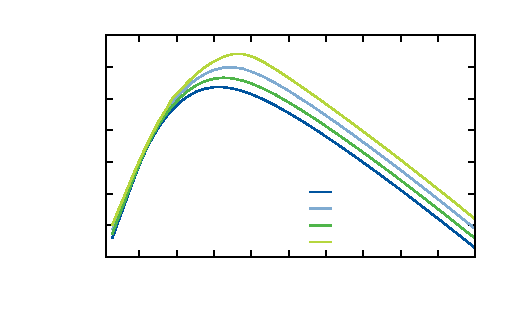
\includegraphics{GNUPlot/pr_isenthalpes}}%
    \gplfronttext
  \end{picture}%
\endgroup

            \caption{Isenthalpes computed by Peng-Robinson EOS.}
            \label{fig:pr_isenthalpes}
        \end{figure}
%        \stdfig{GNUPlot/pr_isenthalpes}{Isenthalpes computed by Peng-Robinson model.}{fig:pr_isenthalpes}{}

        If we employ the Peng-Robinson equation of state, which is appropriate for this mildly non-ideal system
        \cite{AndreasPfennig.2003}, we can plot the isenthalpes for ambient air ($x_{N_2}=0.7812$, $x_{O_2}=0.2095$,
        $x_{Ar}=0.0093$ ) in a PT-diagramm (\figref{fig:pr_isenthalpes}).
        There we can see, that in certain ranges a decrease in pressure at constant enthalpy will result
        in an increase in temperature, while for other regions temperature decreases. It is interesting
        to mention that the non-idealities of a given gas give rise to this effect. For an ideal gas the
        temperature change at isenthalpic expansion would always be zero. Luckily for the cryogenic engineer
        real gases deviate from ideal behaviour especially at elevated pressures and low temperatures \cite{Barron.1985}.
        It is therefore important to give some consideration to the thermodynamic model used to describe the properties
        of the system in question, as the non-ideal properties need to be captured appropriately.

        A different way of expanding a compressed gas, is by letting it produce work in an fluid kinetic machine.
        If one assumes an adiabatic devices and disregards irreversible effects, this process can be viewed as
        isentropic. Analogous to the isenthalpic case an isentropic expansion coefficient can be defined
        \Eq{}{
            \mu_S = \left( \fracddpart{T}{p} \right)_S = \frac{T}{c_p} \left( \fracddpart{v}{T} \right)_p.
        }%
        \ncg{\mu_S}{isentropic expansion coefficient}{\frac{K}{Pa}}

        Here the derivative in the second form corresponds to the volumetric coefficient of thermal expansion
        $\beta$, which is always positive for gases, which in turn means, that an isentropic expansion
        will always result in an temperature decrease, whereas the isenthalpic expansion only led to a decrease for
        specific conditions. Furthermore an isentropic expansion over the same pressure range will always result in
        lower temperatures than an isenthalpic expansion. The reason that isentropic valves are most commonly used
        in liquefaction systems, is that those work producing machines cannot handle significant phase changes,
        which is after all the desired result of liquefaction.

        Traditionally only the isenthalpic expansion had been used within the cryogenic air separation process,
        since -- as mentioned before -- the air needs to be liquefied in order to be fed into be distilled. However
        in modern process configurations the isentropic expansion is also considered to recover some of energy
        form the compression.
